% Created by tikzDevice version 0.6.2-92-0ad2792 on 2013-03-06 19:49:18
% !TEX encoding = UTF-8 Unicode
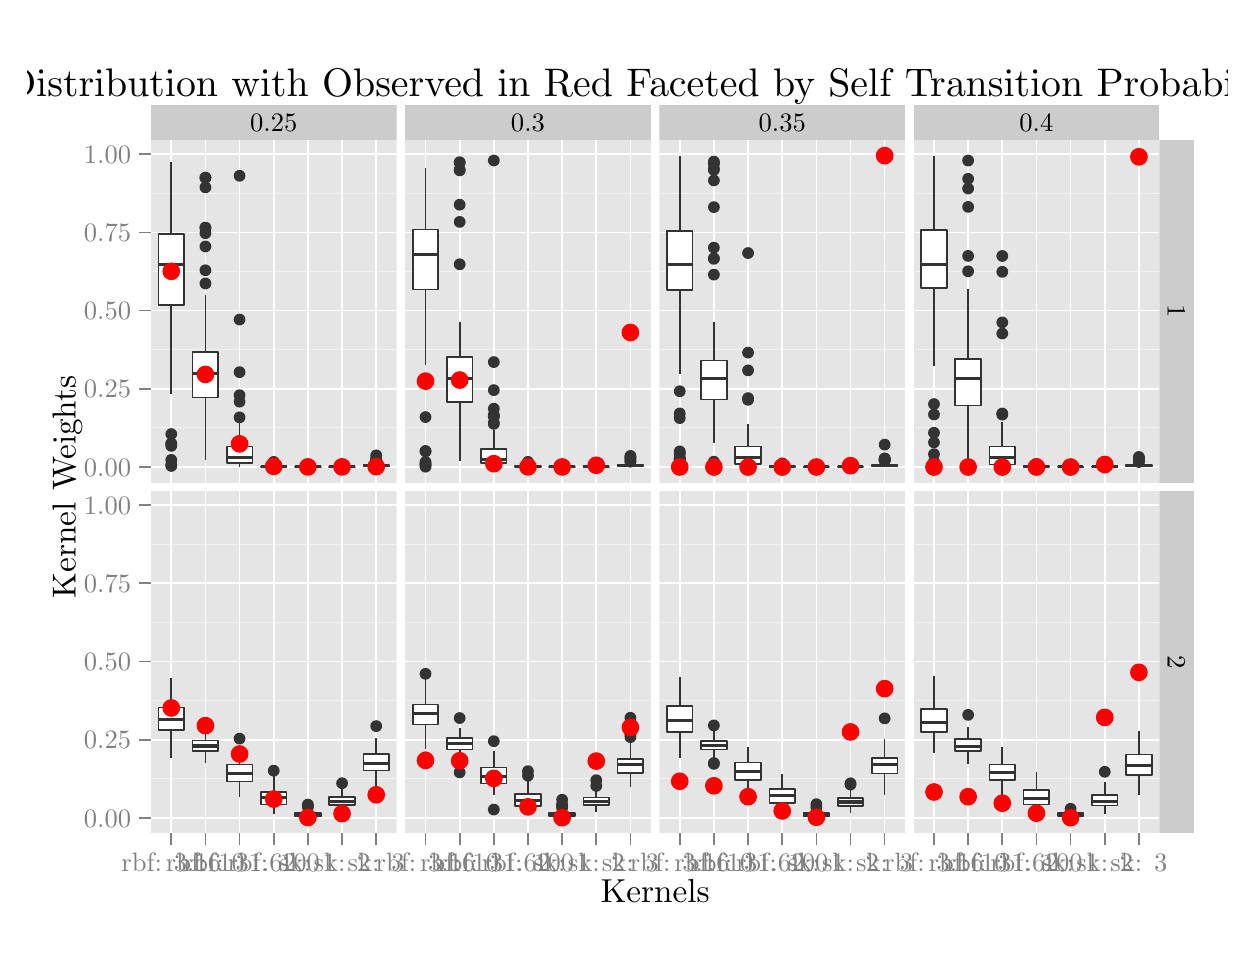
\begin{tikzpicture}[x=1pt,y=1pt]
\definecolor[named]{fillColor}{rgb}{1.00,1.00,1.00}
\path[use as bounding box,fill=fillColor,fill opacity=0.00] (0,0) rectangle (433.62,325.21);
\begin{scope}
\path[clip] (  0.00,  0.00) rectangle (433.62,325.21);
\definecolor[named]{drawColor}{rgb}{1.00,1.00,1.00}
\definecolor[named]{fillColor}{rgb}{1.00,1.00,1.00}

\path[draw=drawColor,line width= 0.6pt,line join=round,line cap=round,fill=fillColor] (  0.00,  0.00) rectangle (433.62,325.21);
\end{scope}
\begin{scope}
\path[clip] ( 44.49,284.60) rectangle (133.34,297.23);
\definecolor[named]{fillColor}{rgb}{0.80,0.80,0.80}

\path[fill=fillColor] ( 44.49,284.60) rectangle (133.34,297.23);
\definecolor[named]{drawColor}{rgb}{0.00,0.00,0.00}

\node[text=drawColor,anchor=base,inner sep=0pt, outer sep=0pt, scale=  0.96] at ( 88.91,287.61) {0.25};
\end{scope}
\begin{scope}
\path[clip] (136.35,284.60) rectangle (225.21,297.23);
\definecolor[named]{fillColor}{rgb}{0.80,0.80,0.80}

\path[fill=fillColor] (136.35,284.60) rectangle (225.21,297.23);
\definecolor[named]{drawColor}{rgb}{0.00,0.00,0.00}

\node[text=drawColor,anchor=base,inner sep=0pt, outer sep=0pt, scale=  0.96] at (180.78,287.61) {0.3};
\end{scope}
\begin{scope}
\path[clip] (228.22,284.60) rectangle (317.07,297.23);
\definecolor[named]{fillColor}{rgb}{0.80,0.80,0.80}

\path[fill=fillColor] (228.22,284.60) rectangle (317.07,297.23);
\definecolor[named]{drawColor}{rgb}{0.00,0.00,0.00}

\node[text=drawColor,anchor=base,inner sep=0pt, outer sep=0pt, scale=  0.96] at (272.65,287.61) {0.35};
\end{scope}
\begin{scope}
\path[clip] (320.09,284.60) rectangle (408.94,297.23);
\definecolor[named]{fillColor}{rgb}{0.80,0.80,0.80}

\path[fill=fillColor] (320.09,284.60) rectangle (408.94,297.23);
\definecolor[named]{drawColor}{rgb}{0.00,0.00,0.00}

\node[text=drawColor,anchor=base,inner sep=0pt, outer sep=0pt, scale=  0.96] at (364.51,287.61) {0.4};
\end{scope}
\begin{scope}
\path[clip] ( 44.49,160.82) rectangle (133.34,284.60);
\definecolor[named]{fillColor}{rgb}{0.90,0.90,0.90}

\path[fill=fillColor] ( 44.49,160.82) rectangle (133.34,284.60);
\definecolor[named]{drawColor}{rgb}{0.95,0.95,0.95}

\path[draw=drawColor,line width= 0.3pt,line join=round] ( 44.49,180.58) --
	(133.34,180.58);

\path[draw=drawColor,line width= 0.3pt,line join=round] ( 44.49,208.84) --
	(133.34,208.84);

\path[draw=drawColor,line width= 0.3pt,line join=round] ( 44.49,237.10) --
	(133.34,237.10);

\path[draw=drawColor,line width= 0.3pt,line join=round] ( 44.49,265.36) --
	(133.34,265.36);
\definecolor[named]{drawColor}{rgb}{1.00,1.00,1.00}

\path[draw=drawColor,line width= 0.6pt,line join=round] ( 44.49,166.45) --
	(133.34,166.45);

\path[draw=drawColor,line width= 0.6pt,line join=round] ( 44.49,194.71) --
	(133.34,194.71);

\path[draw=drawColor,line width= 0.6pt,line join=round] ( 44.49,222.97) --
	(133.34,222.97);

\path[draw=drawColor,line width= 0.6pt,line join=round] ( 44.49,251.23) --
	(133.34,251.23);

\path[draw=drawColor,line width= 0.6pt,line join=round] ( 44.49,279.49) --
	(133.34,279.49);

\path[draw=drawColor,line width= 0.6pt,line join=round] ( 51.89,160.82) --
	( 51.89,284.60);

\path[draw=drawColor,line width= 0.6pt,line join=round] ( 64.23,160.82) --
	( 64.23,284.60);

\path[draw=drawColor,line width= 0.6pt,line join=round] ( 76.57,160.82) --
	( 76.57,284.60);

\path[draw=drawColor,line width= 0.6pt,line join=round] ( 88.91,160.82) --
	( 88.91,284.60);

\path[draw=drawColor,line width= 0.6pt,line join=round] (101.25,160.82) --
	(101.25,284.60);

\path[draw=drawColor,line width= 0.6pt,line join=round] (113.60,160.82) --
	(113.60,284.60);

\path[draw=drawColor,line width= 0.6pt,line join=round] (125.94,160.82) --
	(125.94,284.60);
\definecolor[named]{fillColor}{rgb}{0.20,0.20,0.20}

\path[fill=fillColor] ( 51.89,169.02) circle (  2.13);

\path[fill=fillColor] ( 51.89,167.29) circle (  2.13);

\path[fill=fillColor] ( 51.89,178.35) circle (  2.13);

\path[fill=fillColor] ( 51.89,166.84) circle (  2.13);

\path[fill=fillColor] ( 51.89,174.92) circle (  2.13);

\path[fill=fillColor] ( 51.89,174.86) circle (  2.13);

\path[fill=fillColor] ( 51.89,174.09) circle (  2.13);
\definecolor[named]{drawColor}{rgb}{0.20,0.20,0.20}

\path[draw=drawColor,line width= 0.6pt,line join=round,fill=fillColor] ( 51.89,250.57) -- ( 51.89,276.78);

\path[draw=drawColor,line width= 0.6pt,line join=round,fill=fillColor] ( 51.89,225.08) -- ( 51.89,192.74);
\definecolor[named]{fillColor}{rgb}{1.00,1.00,1.00}

\path[draw=drawColor,line width= 0.6pt,line join=round,line cap=round,fill=fillColor] ( 47.26,250.57) --
	( 47.26,225.08) --
	( 56.52,225.08) --
	( 56.52,250.57) --
	( 47.26,250.57) --
	cycle;
\definecolor[named]{fillColor}{rgb}{0.20,0.20,0.20}

\path[draw=drawColor,line width= 1.1pt,line join=round,fill=fillColor] ( 47.26,239.51) -- ( 56.52,239.51);

\path[fill=fillColor] ( 64.23,250.94) circle (  2.13);

\path[fill=fillColor] ( 64.23,246.14) circle (  2.13);

\path[fill=fillColor] ( 64.23,232.79) circle (  2.13);

\path[fill=fillColor] ( 64.23,267.51) circle (  2.13);

\path[fill=fillColor] ( 64.23,270.96) circle (  2.13);

\path[fill=fillColor] ( 64.23,252.91) circle (  2.13);

\path[fill=fillColor] ( 64.23,271.03) circle (  2.13);

\path[fill=fillColor] ( 64.23,237.54) circle (  2.13);

\path[fill=fillColor] ( 64.23,252.94) circle (  2.13);

\path[draw=drawColor,line width= 0.6pt,line join=round,fill=fillColor] ( 64.23,208.07) -- ( 64.23,228.66);

\path[draw=drawColor,line width= 0.6pt,line join=round,fill=fillColor] ( 64.23,191.59) -- ( 64.23,169.10);
\definecolor[named]{fillColor}{rgb}{1.00,1.00,1.00}

\path[draw=drawColor,line width= 0.6pt,line join=round,line cap=round,fill=fillColor] ( 59.60,208.07) --
	( 59.60,191.59) --
	( 68.86,191.59) --
	( 68.86,208.07) --
	( 59.60,208.07) --
	cycle;
\definecolor[named]{fillColor}{rgb}{0.20,0.20,0.20}

\path[draw=drawColor,line width= 1.1pt,line join=round,fill=fillColor] ( 59.60,200.21) -- ( 68.86,200.21);

\path[fill=fillColor] ( 76.57,192.40) circle (  2.13);

\path[fill=fillColor] ( 76.57,219.74) circle (  2.13);

\path[fill=fillColor] ( 76.57,190.07) circle (  2.13);

\path[fill=fillColor] ( 76.57,184.39) circle (  2.13);

\path[fill=fillColor] ( 76.57,271.68) circle (  2.13);

\path[fill=fillColor] ( 76.57,200.73) circle (  2.13);

\path[draw=drawColor,line width= 0.6pt,line join=round,fill=fillColor] ( 76.57,173.85) -- ( 76.57,182.22);

\path[draw=drawColor,line width= 0.6pt,line join=round,fill=fillColor] ( 76.57,167.93) -- ( 76.57,166.46);
\definecolor[named]{fillColor}{rgb}{1.00,1.00,1.00}

\path[draw=drawColor,line width= 0.6pt,line join=round,line cap=round,fill=fillColor] ( 71.94,173.85) --
	( 71.94,167.93) --
	( 81.20,167.93) --
	( 81.20,173.85) --
	( 71.94,173.85) --
	cycle;
\definecolor[named]{fillColor}{rgb}{0.20,0.20,0.20}

\path[draw=drawColor,line width= 1.1pt,line join=round,fill=fillColor] ( 71.94,169.75) -- ( 81.20,169.75);

\path[fill=fillColor] ( 88.91,167.09) circle (  2.13);

\path[fill=fillColor] ( 88.91,167.06) circle (  2.13);

\path[fill=fillColor] ( 88.91,166.96) circle (  2.13);

\path[fill=fillColor] ( 88.91,166.97) circle (  2.13);

\path[fill=fillColor] ( 88.91,168.30) circle (  2.13);

\path[fill=fillColor] ( 88.91,167.37) circle (  2.13);

\path[fill=fillColor] ( 88.91,167.30) circle (  2.13);

\path[fill=fillColor] ( 88.91,167.20) circle (  2.13);

\path[fill=fillColor] ( 88.91,167.06) circle (  2.13);

\path[fill=fillColor] ( 88.91,166.99) circle (  2.13);

\path[draw=drawColor,line width= 0.6pt,line join=round,fill=fillColor] ( 88.91,166.69) -- ( 88.91,166.94);

\path[draw=drawColor,line width= 0.6pt,line join=round,fill=fillColor] ( 88.91,166.50) -- ( 88.91,166.45);
\definecolor[named]{fillColor}{rgb}{1.00,1.00,1.00}

\path[draw=drawColor,line width= 0.6pt,line join=round,line cap=round,fill=fillColor] ( 84.29,166.69) --
	( 84.29,166.50) --
	( 93.54,166.50) --
	( 93.54,166.69) --
	( 84.29,166.69) --
	cycle;
\definecolor[named]{fillColor}{rgb}{0.20,0.20,0.20}

\path[draw=drawColor,line width= 1.1pt,line join=round,fill=fillColor] ( 84.29,166.59) -- ( 93.54,166.59);

\path[fill=fillColor] (101.25,166.61) circle (  2.13);

\path[draw=drawColor,line width= 0.6pt,line join=round,fill=fillColor] (101.25,166.52) -- (101.25,166.58);

\path[draw=drawColor,line width= 0.6pt,line join=round,fill=fillColor] (101.25,166.46) -- (101.25,166.45);
\definecolor[named]{fillColor}{rgb}{1.00,1.00,1.00}

\path[draw=drawColor,line width= 0.6pt,line join=round,line cap=round,fill=fillColor] ( 96.63,166.52) --
	( 96.63,166.46) --
	(105.88,166.46) --
	(105.88,166.52) --
	( 96.63,166.52) --
	cycle;
\definecolor[named]{fillColor}{rgb}{0.20,0.20,0.20}

\path[draw=drawColor,line width= 1.1pt,line join=round,fill=fillColor] ( 96.63,166.50) -- (105.88,166.50);

\path[fill=fillColor] (113.60,166.69) circle (  2.13);

\path[draw=drawColor,line width= 0.6pt,line join=round,fill=fillColor] (113.60,166.56) -- (113.60,166.69);

\path[draw=drawColor,line width= 0.6pt,line join=round,fill=fillColor] (113.60,166.48) -- (113.60,166.45);
\definecolor[named]{fillColor}{rgb}{1.00,1.00,1.00}

\path[draw=drawColor,line width= 0.6pt,line join=round,line cap=round,fill=fillColor] (108.97,166.56) --
	(108.97,166.48) --
	(118.22,166.48) --
	(118.22,166.56) --
	(108.97,166.56) --
	cycle;
\definecolor[named]{fillColor}{rgb}{0.20,0.20,0.20}

\path[draw=drawColor,line width= 1.1pt,line join=round,fill=fillColor] (108.97,166.52) -- (118.22,166.52);

\path[fill=fillColor] (125.94,168.43) circle (  2.13);

\path[fill=fillColor] (125.94,168.93) circle (  2.13);

\path[fill=fillColor] (125.94,168.02) circle (  2.13);

\path[fill=fillColor] (125.94,168.41) circle (  2.13);

\path[fill=fillColor] (125.94,168.81) circle (  2.13);

\path[fill=fillColor] (125.94,170.66) circle (  2.13);

\path[fill=fillColor] (125.94,168.94) circle (  2.13);

\path[fill=fillColor] (125.94,169.49) circle (  2.13);

\path[draw=drawColor,line width= 0.6pt,line join=round,fill=fillColor] (125.94,167.11) -- (125.94,167.63);

\path[draw=drawColor,line width= 0.6pt,line join=round,fill=fillColor] (125.94,166.58) -- (125.94,166.45);
\definecolor[named]{fillColor}{rgb}{1.00,1.00,1.00}

\path[draw=drawColor,line width= 0.6pt,line join=round,line cap=round,fill=fillColor] (121.31,167.11) --
	(121.31,166.58) --
	(130.56,166.58) --
	(130.56,167.11) --
	(121.31,167.11) --
	cycle;
\definecolor[named]{fillColor}{rgb}{0.20,0.20,0.20}

\path[draw=drawColor,line width= 1.1pt,line join=round,fill=fillColor] (121.31,166.83) -- (130.56,166.83);
\definecolor[named]{fillColor}{rgb}{1.00,0.00,0.00}

\path[fill=fillColor] ( 51.89,237.17) circle (  3.20);

\path[fill=fillColor] ( 64.23,199.91) circle (  3.20);

\path[fill=fillColor] ( 76.57,174.82) circle (  3.20);

\path[fill=fillColor] ( 88.91,166.69) circle (  3.20);

\path[fill=fillColor] (101.25,166.49) circle (  3.20);

\path[fill=fillColor] (113.60,166.50) circle (  3.20);

\path[fill=fillColor] (125.94,166.59) circle (  3.20);
\end{scope}
\begin{scope}
\path[clip] ( 44.49, 34.03) rectangle (133.34,157.81);
\definecolor[named]{fillColor}{rgb}{0.90,0.90,0.90}

\path[fill=fillColor] ( 44.49, 34.03) rectangle (133.34,157.81);
\definecolor[named]{drawColor}{rgb}{0.95,0.95,0.95}

\path[draw=drawColor,line width= 0.3pt,line join=round] ( 44.49, 53.79) --
	(133.34, 53.79);

\path[draw=drawColor,line width= 0.3pt,line join=round] ( 44.49, 82.05) --
	(133.34, 82.05);

\path[draw=drawColor,line width= 0.3pt,line join=round] ( 44.49,110.31) --
	(133.34,110.31);

\path[draw=drawColor,line width= 0.3pt,line join=round] ( 44.49,138.57) --
	(133.34,138.57);
\definecolor[named]{drawColor}{rgb}{1.00,1.00,1.00}

\path[draw=drawColor,line width= 0.6pt,line join=round] ( 44.49, 39.66) --
	(133.34, 39.66);

\path[draw=drawColor,line width= 0.6pt,line join=round] ( 44.49, 67.92) --
	(133.34, 67.92);

\path[draw=drawColor,line width= 0.6pt,line join=round] ( 44.49, 96.18) --
	(133.34, 96.18);

\path[draw=drawColor,line width= 0.6pt,line join=round] ( 44.49,124.44) --
	(133.34,124.44);

\path[draw=drawColor,line width= 0.6pt,line join=round] ( 44.49,152.70) --
	(133.34,152.70);

\path[draw=drawColor,line width= 0.6pt,line join=round] ( 51.89, 34.03) --
	( 51.89,157.81);

\path[draw=drawColor,line width= 0.6pt,line join=round] ( 64.23, 34.03) --
	( 64.23,157.81);

\path[draw=drawColor,line width= 0.6pt,line join=round] ( 76.57, 34.03) --
	( 76.57,157.81);

\path[draw=drawColor,line width= 0.6pt,line join=round] ( 88.91, 34.03) --
	( 88.91,157.81);

\path[draw=drawColor,line width= 0.6pt,line join=round] (101.25, 34.03) --
	(101.25,157.81);

\path[draw=drawColor,line width= 0.6pt,line join=round] (113.60, 34.03) --
	(113.60,157.81);

\path[draw=drawColor,line width= 0.6pt,line join=round] (125.94, 34.03) --
	(125.94,157.81);
\definecolor[named]{drawColor}{rgb}{0.20,0.20,0.20}
\definecolor[named]{fillColor}{rgb}{0.20,0.20,0.20}

\path[draw=drawColor,line width= 0.6pt,line join=round,fill=fillColor] ( 51.89, 79.51) -- ( 51.89, 90.25);

\path[draw=drawColor,line width= 0.6pt,line join=round,fill=fillColor] ( 51.89, 71.53) -- ( 51.89, 61.30);
\definecolor[named]{fillColor}{rgb}{1.00,1.00,1.00}

\path[draw=drawColor,line width= 0.6pt,line join=round,line cap=round,fill=fillColor] ( 47.26, 79.51) --
	( 47.26, 71.53) --
	( 56.52, 71.53) --
	( 56.52, 79.51) --
	( 47.26, 79.51) --
	cycle;
\definecolor[named]{fillColor}{rgb}{0.20,0.20,0.20}

\path[draw=drawColor,line width= 1.1pt,line join=round,fill=fillColor] ( 47.26, 75.29) -- ( 56.52, 75.29);

\path[draw=drawColor,line width= 0.6pt,line join=round,fill=fillColor] ( 64.23, 67.67) -- ( 64.23, 72.12);

\path[draw=drawColor,line width= 0.6pt,line join=round,fill=fillColor] ( 64.23, 63.92) -- ( 64.23, 59.49);
\definecolor[named]{fillColor}{rgb}{1.00,1.00,1.00}

\path[draw=drawColor,line width= 0.6pt,line join=round,line cap=round,fill=fillColor] ( 59.60, 67.67) --
	( 59.60, 63.92) --
	( 68.86, 63.92) --
	( 68.86, 67.67) --
	( 59.60, 67.67) --
	cycle;
\definecolor[named]{fillColor}{rgb}{0.20,0.20,0.20}

\path[draw=drawColor,line width= 1.1pt,line join=round,fill=fillColor] ( 59.60, 65.64) -- ( 68.86, 65.64);

\path[fill=fillColor] ( 76.57, 68.31) circle (  2.13);

\path[draw=drawColor,line width= 0.6pt,line join=round,fill=fillColor] ( 76.57, 58.93) -- ( 76.57, 65.10);

\path[draw=drawColor,line width= 0.6pt,line join=round,fill=fillColor] ( 76.57, 52.86) -- ( 76.57, 47.35);
\definecolor[named]{fillColor}{rgb}{1.00,1.00,1.00}

\path[draw=drawColor,line width= 0.6pt,line join=round,line cap=round,fill=fillColor] ( 71.94, 58.93) --
	( 71.94, 52.86) --
	( 81.20, 52.86) --
	( 81.20, 58.93) --
	( 71.94, 58.93) --
	cycle;
\definecolor[named]{fillColor}{rgb}{0.20,0.20,0.20}

\path[draw=drawColor,line width= 1.1pt,line join=round,fill=fillColor] ( 71.94, 55.76) -- ( 81.20, 55.76);

\path[fill=fillColor] ( 88.91, 56.72) circle (  2.13);

\path[draw=drawColor,line width= 0.6pt,line join=round,fill=fillColor] ( 88.91, 48.95) -- ( 88.91, 55.48);

\path[draw=drawColor,line width= 0.6pt,line join=round,fill=fillColor] ( 88.91, 44.50) -- ( 88.91, 41.08);
\definecolor[named]{fillColor}{rgb}{1.00,1.00,1.00}

\path[draw=drawColor,line width= 0.6pt,line join=round,line cap=round,fill=fillColor] ( 84.29, 48.95) --
	( 84.29, 44.50) --
	( 93.54, 44.50) --
	( 93.54, 48.95) --
	( 84.29, 48.95) --
	cycle;
\definecolor[named]{fillColor}{rgb}{0.20,0.20,0.20}

\path[draw=drawColor,line width= 1.1pt,line join=round,fill=fillColor] ( 84.29, 46.90) -- ( 93.54, 46.90);

\path[fill=fillColor] (101.25, 43.86) circle (  2.13);

\path[fill=fillColor] (101.25, 44.48) circle (  2.13);

\path[fill=fillColor] (101.25, 43.68) circle (  2.13);

\path[draw=drawColor,line width= 0.6pt,line join=round,fill=fillColor] (101.25, 41.52) -- (101.25, 43.32);

\path[draw=drawColor,line width= 0.6pt,line join=round,fill=fillColor] (101.25, 40.22) -- (101.25, 39.75);
\definecolor[named]{fillColor}{rgb}{1.00,1.00,1.00}

\path[draw=drawColor,line width= 0.6pt,line join=round,line cap=round,fill=fillColor] ( 96.63, 41.52) --
	( 96.63, 40.22) --
	(105.88, 40.22) --
	(105.88, 41.52) --
	( 96.63, 41.52) --
	cycle;
\definecolor[named]{fillColor}{rgb}{0.20,0.20,0.20}

\path[draw=drawColor,line width= 1.1pt,line join=round,fill=fillColor] ( 96.63, 40.92) -- (105.88, 40.92);

\path[fill=fillColor] (113.60, 52.19) circle (  2.13);

\path[draw=drawColor,line width= 0.6pt,line join=round,fill=fillColor] (113.60, 47.21) -- (113.60, 51.49);

\path[draw=drawColor,line width= 0.6pt,line join=round,fill=fillColor] (113.60, 44.31) -- (113.60, 41.61);
\definecolor[named]{fillColor}{rgb}{1.00,1.00,1.00}

\path[draw=drawColor,line width= 0.6pt,line join=round,line cap=round,fill=fillColor] (108.97, 47.21) --
	(108.97, 44.31) --
	(118.22, 44.31) --
	(118.22, 47.21) --
	(108.97, 47.21) --
	cycle;
\definecolor[named]{fillColor}{rgb}{0.20,0.20,0.20}

\path[draw=drawColor,line width= 1.1pt,line join=round,fill=fillColor] (108.97, 45.45) -- (118.22, 45.45);

\path[fill=fillColor] (125.94, 72.83) circle (  2.13);

\path[draw=drawColor,line width= 0.6pt,line join=round,fill=fillColor] (125.94, 62.68) -- (125.94, 68.59);

\path[draw=drawColor,line width= 0.6pt,line join=round,fill=fillColor] (125.94, 56.77) -- (125.94, 50.73);
\definecolor[named]{fillColor}{rgb}{1.00,1.00,1.00}

\path[draw=drawColor,line width= 0.6pt,line join=round,line cap=round,fill=fillColor] (121.31, 62.68) --
	(121.31, 56.77) --
	(130.56, 56.77) --
	(130.56, 62.68) --
	(121.31, 62.68) --
	cycle;
\definecolor[named]{fillColor}{rgb}{0.20,0.20,0.20}

\path[draw=drawColor,line width= 1.1pt,line join=round,fill=fillColor] (121.31, 59.28) -- (130.56, 59.28);
\definecolor[named]{fillColor}{rgb}{1.00,0.00,0.00}

\path[fill=fillColor] ( 51.89, 79.39) circle (  3.20);

\path[fill=fillColor] ( 64.23, 73.01) circle (  3.20);

\path[fill=fillColor] ( 76.57, 62.75) circle (  3.20);

\path[fill=fillColor] ( 88.91, 46.47) circle (  3.20);

\path[fill=fillColor] (101.25, 39.80) circle (  3.20);

\path[fill=fillColor] (113.60, 41.22) circle (  3.20);

\path[fill=fillColor] (125.94, 48.02) circle (  3.20);
\end{scope}
\begin{scope}
\path[clip] (136.35,160.82) rectangle (225.21,284.60);
\definecolor[named]{fillColor}{rgb}{0.90,0.90,0.90}

\path[fill=fillColor] (136.35,160.82) rectangle (225.21,284.60);
\definecolor[named]{drawColor}{rgb}{0.95,0.95,0.95}

\path[draw=drawColor,line width= 0.3pt,line join=round] (136.35,180.58) --
	(225.21,180.58);

\path[draw=drawColor,line width= 0.3pt,line join=round] (136.35,208.84) --
	(225.21,208.84);

\path[draw=drawColor,line width= 0.3pt,line join=round] (136.35,237.10) --
	(225.21,237.10);

\path[draw=drawColor,line width= 0.3pt,line join=round] (136.35,265.36) --
	(225.21,265.36);
\definecolor[named]{drawColor}{rgb}{1.00,1.00,1.00}

\path[draw=drawColor,line width= 0.6pt,line join=round] (136.35,166.45) --
	(225.21,166.45);

\path[draw=drawColor,line width= 0.6pt,line join=round] (136.35,194.71) --
	(225.21,194.71);

\path[draw=drawColor,line width= 0.6pt,line join=round] (136.35,222.97) --
	(225.21,222.97);

\path[draw=drawColor,line width= 0.6pt,line join=round] (136.35,251.23) --
	(225.21,251.23);

\path[draw=drawColor,line width= 0.6pt,line join=round] (136.35,279.49) --
	(225.21,279.49);

\path[draw=drawColor,line width= 0.6pt,line join=round] (143.76,160.82) --
	(143.76,284.60);

\path[draw=drawColor,line width= 0.6pt,line join=round] (156.10,160.82) --
	(156.10,284.60);

\path[draw=drawColor,line width= 0.6pt,line join=round] (168.44,160.82) --
	(168.44,284.60);

\path[draw=drawColor,line width= 0.6pt,line join=round] (180.78,160.82) --
	(180.78,284.60);

\path[draw=drawColor,line width= 0.6pt,line join=round] (193.12,160.82) --
	(193.12,284.60);

\path[draw=drawColor,line width= 0.6pt,line join=round] (205.46,160.82) --
	(205.46,284.60);

\path[draw=drawColor,line width= 0.6pt,line join=round] (217.80,160.82) --
	(217.80,284.60);
\definecolor[named]{fillColor}{rgb}{0.20,0.20,0.20}

\path[fill=fillColor] (143.76,172.07) circle (  2.13);

\path[fill=fillColor] (143.76,166.57) circle (  2.13);

\path[fill=fillColor] (143.76,167.33) circle (  2.13);

\path[fill=fillColor] (143.76,167.25) circle (  2.13);

\path[fill=fillColor] (143.76,172.25) circle (  2.13);

\path[fill=fillColor] (143.76,184.49) circle (  2.13);

\path[fill=fillColor] (143.76,168.30) circle (  2.13);

\path[fill=fillColor] (143.76,167.77) circle (  2.13);
\definecolor[named]{drawColor}{rgb}{0.20,0.20,0.20}

\path[draw=drawColor,line width= 0.6pt,line join=round,fill=fillColor] (143.76,252.22) -- (143.76,274.35);

\path[draw=drawColor,line width= 0.6pt,line join=round,fill=fillColor] (143.76,230.59) -- (143.76,203.36);
\definecolor[named]{fillColor}{rgb}{1.00,1.00,1.00}

\path[draw=drawColor,line width= 0.6pt,line join=round,line cap=round,fill=fillColor] (139.13,252.22) --
	(139.13,230.59) --
	(148.38,230.59) --
	(148.38,252.22) --
	(139.13,252.22) --
	cycle;
\definecolor[named]{fillColor}{rgb}{0.20,0.20,0.20}

\path[draw=drawColor,line width= 1.1pt,line join=round,fill=fillColor] (139.13,243.27) -- (148.38,243.27);

\path[fill=fillColor] (156.10,255.03) circle (  2.13);

\path[fill=fillColor] (156.10,276.55) circle (  2.13);

\path[fill=fillColor] (156.10,273.89) circle (  2.13);

\path[fill=fillColor] (156.10,273.64) circle (  2.13);

\path[fill=fillColor] (156.10,261.24) circle (  2.13);

\path[fill=fillColor] (156.10,239.70) circle (  2.13);

\path[fill=fillColor] (156.10,276.50) circle (  2.13);

\path[draw=drawColor,line width= 0.6pt,line join=round,fill=fillColor] (156.10,206.25) -- (156.10,218.84);

\path[draw=drawColor,line width= 0.6pt,line join=round,fill=fillColor] (156.10,189.95) -- (156.10,168.56);
\definecolor[named]{fillColor}{rgb}{1.00,1.00,1.00}

\path[draw=drawColor,line width= 0.6pt,line join=round,line cap=round,fill=fillColor] (151.47,206.25) --
	(151.47,189.95) --
	(160.73,189.95) --
	(160.73,206.25) --
	(151.47,206.25) --
	cycle;
\definecolor[named]{fillColor}{rgb}{0.20,0.20,0.20}

\path[draw=drawColor,line width= 1.1pt,line join=round,fill=fillColor] (151.47,198.27) -- (160.73,198.27);

\path[fill=fillColor] (168.44,194.24) circle (  2.13);

\path[fill=fillColor] (168.44,185.24) circle (  2.13);

\path[fill=fillColor] (168.44,277.21) circle (  2.13);

\path[fill=fillColor] (168.44,182.40) circle (  2.13);

\path[fill=fillColor] (168.44,187.51) circle (  2.13);

\path[fill=fillColor] (168.44,182.04) circle (  2.13);

\path[fill=fillColor] (168.44,184.72) circle (  2.13);

\path[fill=fillColor] (168.44,204.37) circle (  2.13);

\path[fill=fillColor] (168.44,184.77) circle (  2.13);

\path[draw=drawColor,line width= 0.6pt,line join=round,fill=fillColor] (168.44,173.02) -- (168.44,179.96);

\path[draw=drawColor,line width= 0.6pt,line join=round,fill=fillColor] (168.44,167.99) -- (168.44,166.46);
\definecolor[named]{fillColor}{rgb}{1.00,1.00,1.00}

\path[draw=drawColor,line width= 0.6pt,line join=round,line cap=round,fill=fillColor] (163.81,173.02) --
	(163.81,167.99) --
	(173.07,167.99) --
	(173.07,173.02) --
	(163.81,173.02) --
	cycle;
\definecolor[named]{fillColor}{rgb}{0.20,0.20,0.20}

\path[draw=drawColor,line width= 1.1pt,line join=round,fill=fillColor] (163.81,169.28) -- (173.07,169.28);

\path[fill=fillColor] (180.78,168.31) circle (  2.13);

\path[fill=fillColor] (180.78,166.97) circle (  2.13);

\path[fill=fillColor] (180.78,167.00) circle (  2.13);

\path[fill=fillColor] (180.78,167.08) circle (  2.13);

\path[fill=fillColor] (180.78,166.97) circle (  2.13);

\path[fill=fillColor] (180.78,167.28) circle (  2.13);

\path[fill=fillColor] (180.78,166.96) circle (  2.13);

\path[fill=fillColor] (180.78,167.69) circle (  2.13);

\path[fill=fillColor] (180.78,167.04) circle (  2.13);

\path[fill=fillColor] (180.78,167.31) circle (  2.13);

\path[fill=fillColor] (180.78,167.59) circle (  2.13);

\path[fill=fillColor] (180.78,167.04) circle (  2.13);

\path[draw=drawColor,line width= 0.6pt,line join=round,fill=fillColor] (180.78,166.70) -- (180.78,166.91);

\path[draw=drawColor,line width= 0.6pt,line join=round,fill=fillColor] (180.78,166.54) -- (180.78,166.45);
\definecolor[named]{fillColor}{rgb}{1.00,1.00,1.00}

\path[draw=drawColor,line width= 0.6pt,line join=round,line cap=round,fill=fillColor] (176.15,166.70) --
	(176.15,166.54) --
	(185.41,166.54) --
	(185.41,166.70) --
	(176.15,166.70) --
	cycle;
\definecolor[named]{fillColor}{rgb}{0.20,0.20,0.20}

\path[draw=drawColor,line width= 1.1pt,line join=round,fill=fillColor] (176.15,166.59) -- (185.41,166.59);

\path[draw=drawColor,line width= 0.6pt,line join=round,fill=fillColor] (193.12,166.52) -- (193.12,166.59);

\path[draw=drawColor,line width= 0.6pt,line join=round,fill=fillColor] (193.12,166.47) -- (193.12,166.45);
\definecolor[named]{fillColor}{rgb}{1.00,1.00,1.00}

\path[draw=drawColor,line width= 0.6pt,line join=round,line cap=round,fill=fillColor] (188.49,166.52) --
	(188.49,166.47) --
	(197.75,166.47) --
	(197.75,166.52) --
	(188.49,166.52) --
	cycle;
\definecolor[named]{fillColor}{rgb}{0.20,0.20,0.20}

\path[draw=drawColor,line width= 1.1pt,line join=round,fill=fillColor] (188.49,166.50) -- (197.75,166.50);

\path[draw=drawColor,line width= 0.6pt,line join=round,fill=fillColor] (205.46,166.57) -- (205.46,166.68);

\path[draw=drawColor,line width= 0.6pt,line join=round,fill=fillColor] (205.46,166.49) -- (205.46,166.45);
\definecolor[named]{fillColor}{rgb}{1.00,1.00,1.00}

\path[draw=drawColor,line width= 0.6pt,line join=round,line cap=round,fill=fillColor] (200.83,166.57) --
	(200.83,166.49) --
	(210.09,166.49) --
	(210.09,166.57) --
	(200.83,166.57) --
	cycle;
\definecolor[named]{fillColor}{rgb}{0.20,0.20,0.20}

\path[draw=drawColor,line width= 1.1pt,line join=round,fill=fillColor] (200.83,166.54) -- (210.09,166.54);

\path[fill=fillColor] (217.80,168.56) circle (  2.13);

\path[fill=fillColor] (217.80,168.39) circle (  2.13);

\path[fill=fillColor] (217.80,169.34) circle (  2.13);

\path[fill=fillColor] (217.80,170.18) circle (  2.13);

\path[fill=fillColor] (217.80,170.46) circle (  2.13);

\path[fill=fillColor] (217.80,169.72) circle (  2.13);

\path[draw=drawColor,line width= 0.6pt,line join=round,fill=fillColor] (217.80,167.32) -- (217.80,168.28);

\path[draw=drawColor,line width= 0.6pt,line join=round,fill=fillColor] (217.80,166.64) -- (217.80,166.45);
\definecolor[named]{fillColor}{rgb}{1.00,1.00,1.00}

\path[draw=drawColor,line width= 0.6pt,line join=round,line cap=round,fill=fillColor] (213.17,167.32) --
	(213.17,166.64) --
	(222.43,166.64) --
	(222.43,167.32) --
	(213.17,167.32) --
	cycle;
\definecolor[named]{fillColor}{rgb}{0.20,0.20,0.20}

\path[draw=drawColor,line width= 1.1pt,line join=round,fill=fillColor] (213.17,166.90) -- (222.43,166.90);
\definecolor[named]{fillColor}{rgb}{1.00,0.00,0.00}

\path[fill=fillColor] (143.76,197.48) circle (  3.20);

\path[fill=fillColor] (156.10,197.88) circle (  3.20);

\path[fill=fillColor] (168.44,167.66) circle (  3.20);

\path[fill=fillColor] (180.78,166.51) circle (  3.20);

\path[fill=fillColor] (193.12,166.48) circle (  3.20);

\path[fill=fillColor] (205.46,167.08) circle (  3.20);

\path[fill=fillColor] (217.80,215.07) circle (  3.20);
\end{scope}
\begin{scope}
\path[clip] (136.35, 34.03) rectangle (225.21,157.81);
\definecolor[named]{fillColor}{rgb}{0.90,0.90,0.90}

\path[fill=fillColor] (136.35, 34.03) rectangle (225.21,157.81);
\definecolor[named]{drawColor}{rgb}{0.95,0.95,0.95}

\path[draw=drawColor,line width= 0.3pt,line join=round] (136.35, 53.79) --
	(225.21, 53.79);

\path[draw=drawColor,line width= 0.3pt,line join=round] (136.35, 82.05) --
	(225.21, 82.05);

\path[draw=drawColor,line width= 0.3pt,line join=round] (136.35,110.31) --
	(225.21,110.31);

\path[draw=drawColor,line width= 0.3pt,line join=round] (136.35,138.57) --
	(225.21,138.57);
\definecolor[named]{drawColor}{rgb}{1.00,1.00,1.00}

\path[draw=drawColor,line width= 0.6pt,line join=round] (136.35, 39.66) --
	(225.21, 39.66);

\path[draw=drawColor,line width= 0.6pt,line join=round] (136.35, 67.92) --
	(225.21, 67.92);

\path[draw=drawColor,line width= 0.6pt,line join=round] (136.35, 96.18) --
	(225.21, 96.18);

\path[draw=drawColor,line width= 0.6pt,line join=round] (136.35,124.44) --
	(225.21,124.44);

\path[draw=drawColor,line width= 0.6pt,line join=round] (136.35,152.70) --
	(225.21,152.70);

\path[draw=drawColor,line width= 0.6pt,line join=round] (143.76, 34.03) --
	(143.76,157.81);

\path[draw=drawColor,line width= 0.6pt,line join=round] (156.10, 34.03) --
	(156.10,157.81);

\path[draw=drawColor,line width= 0.6pt,line join=round] (168.44, 34.03) --
	(168.44,157.81);

\path[draw=drawColor,line width= 0.6pt,line join=round] (180.78, 34.03) --
	(180.78,157.81);

\path[draw=drawColor,line width= 0.6pt,line join=round] (193.12, 34.03) --
	(193.12,157.81);

\path[draw=drawColor,line width= 0.6pt,line join=round] (205.46, 34.03) --
	(205.46,157.81);

\path[draw=drawColor,line width= 0.6pt,line join=round] (217.80, 34.03) --
	(217.80,157.81);
\definecolor[named]{fillColor}{rgb}{0.20,0.20,0.20}

\path[fill=fillColor] (143.76, 61.50) circle (  2.13);

\path[fill=fillColor] (143.76, 91.73) circle (  2.13);
\definecolor[named]{drawColor}{rgb}{0.20,0.20,0.20}

\path[draw=drawColor,line width= 0.6pt,line join=round,fill=fillColor] (143.76, 80.60) -- (143.76, 91.05);

\path[draw=drawColor,line width= 0.6pt,line join=round,fill=fillColor] (143.76, 73.37) -- (143.76, 64.72);
\definecolor[named]{fillColor}{rgb}{1.00,1.00,1.00}

\path[draw=drawColor,line width= 0.6pt,line join=round,line cap=round,fill=fillColor] (139.13, 80.60) --
	(139.13, 73.37) --
	(148.38, 73.37) --
	(148.38, 80.60) --
	(139.13, 80.60) --
	cycle;
\definecolor[named]{fillColor}{rgb}{0.20,0.20,0.20}

\path[draw=drawColor,line width= 1.1pt,line join=round,fill=fillColor] (139.13, 77.52) -- (148.38, 77.52);

\path[fill=fillColor] (156.10, 75.74) circle (  2.13);

\path[fill=fillColor] (156.10, 56.11) circle (  2.13);

\path[draw=drawColor,line width= 0.6pt,line join=round,fill=fillColor] (156.10, 68.60) -- (156.10, 72.19);

\path[draw=drawColor,line width= 0.6pt,line join=round,fill=fillColor] (156.10, 64.32) -- (156.10, 58.55);
\definecolor[named]{fillColor}{rgb}{1.00,1.00,1.00}

\path[draw=drawColor,line width= 0.6pt,line join=round,line cap=round,fill=fillColor] (151.47, 68.60) --
	(151.47, 64.32) --
	(160.73, 64.32) --
	(160.73, 68.60) --
	(151.47, 68.60) --
	cycle;
\definecolor[named]{fillColor}{rgb}{0.20,0.20,0.20}

\path[draw=drawColor,line width= 1.1pt,line join=round,fill=fillColor] (151.47, 66.65) -- (160.73, 66.65);

\path[fill=fillColor] (168.44, 67.39) circle (  2.13);

\path[fill=fillColor] (168.44, 42.67) circle (  2.13);

\path[draw=drawColor,line width= 0.6pt,line join=round,fill=fillColor] (168.44, 57.84) -- (168.44, 63.89);

\path[draw=drawColor,line width= 0.6pt,line join=round,fill=fillColor] (168.44, 52.13) -- (168.44, 47.83);
\definecolor[named]{fillColor}{rgb}{1.00,1.00,1.00}

\path[draw=drawColor,line width= 0.6pt,line join=round,line cap=round,fill=fillColor] (163.81, 57.84) --
	(163.81, 52.13) --
	(173.07, 52.13) --
	(173.07, 57.84) --
	(163.81, 57.84) --
	cycle;
\definecolor[named]{fillColor}{rgb}{0.20,0.20,0.20}

\path[draw=drawColor,line width= 1.1pt,line join=round,fill=fillColor] (163.81, 54.65) -- (173.07, 54.65);

\path[fill=fillColor] (180.78, 56.55) circle (  2.13);

\path[fill=fillColor] (180.78, 54.90) circle (  2.13);

\path[draw=drawColor,line width= 0.6pt,line join=round,fill=fillColor] (180.78, 48.36) -- (180.78, 53.64);

\path[draw=drawColor,line width= 0.6pt,line join=round,fill=fillColor] (180.78, 44.02) -- (180.78, 40.73);
\definecolor[named]{fillColor}{rgb}{1.00,1.00,1.00}

\path[draw=drawColor,line width= 0.6pt,line join=round,line cap=round,fill=fillColor] (176.15, 48.36) --
	(176.15, 44.02) --
	(185.41, 44.02) --
	(185.41, 48.36) --
	(176.15, 48.36) --
	cycle;
\definecolor[named]{fillColor}{rgb}{0.20,0.20,0.20}

\path[draw=drawColor,line width= 1.1pt,line join=round,fill=fillColor] (176.15, 45.78) -- (185.41, 45.78);

\path[fill=fillColor] (193.12, 43.35) circle (  2.13);

\path[fill=fillColor] (193.12, 44.37) circle (  2.13);

\path[fill=fillColor] (193.12, 44.42) circle (  2.13);

\path[fill=fillColor] (193.12, 46.22) circle (  2.13);

\path[fill=fillColor] (193.12, 43.66) circle (  2.13);

\path[draw=drawColor,line width= 0.6pt,line join=round,fill=fillColor] (193.12, 41.42) -- (193.12, 43.14);

\path[draw=drawColor,line width= 0.6pt,line join=round,fill=fillColor] (193.12, 40.24) -- (193.12, 39.69);
\definecolor[named]{fillColor}{rgb}{1.00,1.00,1.00}

\path[draw=drawColor,line width= 0.6pt,line join=round,line cap=round,fill=fillColor] (188.49, 41.42) --
	(188.49, 40.24) --
	(197.75, 40.24) --
	(197.75, 41.42) --
	(188.49, 41.42) --
	cycle;
\definecolor[named]{fillColor}{rgb}{0.20,0.20,0.20}

\path[draw=drawColor,line width= 1.1pt,line join=round,fill=fillColor] (188.49, 40.78) -- (197.75, 40.78);

\path[fill=fillColor] (205.46, 51.21) circle (  2.13);

\path[fill=fillColor] (205.46, 53.29) circle (  2.13);

\path[draw=drawColor,line width= 0.6pt,line join=round,fill=fillColor] (205.46, 47.02) -- (205.46, 51.11);

\path[draw=drawColor,line width= 0.6pt,line join=round,fill=fillColor] (205.46, 44.27) -- (205.46, 41.88);
\definecolor[named]{fillColor}{rgb}{1.00,1.00,1.00}

\path[draw=drawColor,line width= 0.6pt,line join=round,line cap=round,fill=fillColor] (200.83, 47.02) --
	(200.83, 44.27) --
	(210.09, 44.27) --
	(210.09, 47.02) --
	(200.83, 47.02) --
	cycle;
\definecolor[named]{fillColor}{rgb}{0.20,0.20,0.20}

\path[draw=drawColor,line width= 1.1pt,line join=round,fill=fillColor] (200.83, 45.56) -- (210.09, 45.56);

\path[fill=fillColor] (217.80, 68.84) circle (  2.13);

\path[fill=fillColor] (217.80, 69.89) circle (  2.13);

\path[fill=fillColor] (217.80, 70.24) circle (  2.13);

\path[fill=fillColor] (217.80, 73.98) circle (  2.13);

\path[fill=fillColor] (217.80, 75.84) circle (  2.13);

\path[draw=drawColor,line width= 0.6pt,line join=round,fill=fillColor] (217.80, 61.05) -- (217.80, 68.62);

\path[draw=drawColor,line width= 0.6pt,line join=round,fill=fillColor] (217.80, 55.93) -- (217.80, 50.73);
\definecolor[named]{fillColor}{rgb}{1.00,1.00,1.00}

\path[draw=drawColor,line width= 0.6pt,line join=round,line cap=round,fill=fillColor] (213.17, 61.05) --
	(213.17, 55.93) --
	(222.43, 55.93) --
	(222.43, 61.05) --
	(213.17, 61.05) --
	cycle;
\definecolor[named]{fillColor}{rgb}{0.20,0.20,0.20}

\path[draw=drawColor,line width= 1.1pt,line join=round,fill=fillColor] (213.17, 58.84) -- (222.43, 58.84);
\definecolor[named]{fillColor}{rgb}{1.00,0.00,0.00}

\path[fill=fillColor] (143.76, 60.44) circle (  3.20);

\path[fill=fillColor] (156.10, 60.31) circle (  3.20);

\path[fill=fillColor] (168.44, 53.94) circle (  3.20);

\path[fill=fillColor] (180.78, 43.66) circle (  3.20);

\path[fill=fillColor] (193.12, 39.74) circle (  3.20);

\path[fill=fillColor] (205.46, 60.19) circle (  3.20);

\path[fill=fillColor] (217.80, 72.38) circle (  3.20);
\end{scope}
\begin{scope}
\path[clip] (228.22,160.82) rectangle (317.07,284.60);
\definecolor[named]{fillColor}{rgb}{0.90,0.90,0.90}

\path[fill=fillColor] (228.22,160.82) rectangle (317.07,284.60);
\definecolor[named]{drawColor}{rgb}{0.95,0.95,0.95}

\path[draw=drawColor,line width= 0.3pt,line join=round] (228.22,180.58) --
	(317.07,180.58);

\path[draw=drawColor,line width= 0.3pt,line join=round] (228.22,208.84) --
	(317.07,208.84);

\path[draw=drawColor,line width= 0.3pt,line join=round] (228.22,237.10) --
	(317.07,237.10);

\path[draw=drawColor,line width= 0.3pt,line join=round] (228.22,265.36) --
	(317.07,265.36);
\definecolor[named]{drawColor}{rgb}{1.00,1.00,1.00}

\path[draw=drawColor,line width= 0.6pt,line join=round] (228.22,166.45) --
	(317.07,166.45);

\path[draw=drawColor,line width= 0.6pt,line join=round] (228.22,194.71) --
	(317.07,194.71);

\path[draw=drawColor,line width= 0.6pt,line join=round] (228.22,222.97) --
	(317.07,222.97);

\path[draw=drawColor,line width= 0.6pt,line join=round] (228.22,251.23) --
	(317.07,251.23);

\path[draw=drawColor,line width= 0.6pt,line join=round] (228.22,279.49) --
	(317.07,279.49);

\path[draw=drawColor,line width= 0.6pt,line join=round] (235.62,160.82) --
	(235.62,284.60);

\path[draw=drawColor,line width= 0.6pt,line join=round] (247.96,160.82) --
	(247.96,284.60);

\path[draw=drawColor,line width= 0.6pt,line join=round] (260.31,160.82) --
	(260.31,284.60);

\path[draw=drawColor,line width= 0.6pt,line join=round] (272.65,160.82) --
	(272.65,284.60);

\path[draw=drawColor,line width= 0.6pt,line join=round] (284.99,160.82) --
	(284.99,284.60);

\path[draw=drawColor,line width= 0.6pt,line join=round] (297.33,160.82) --
	(297.33,284.60);

\path[draw=drawColor,line width= 0.6pt,line join=round] (309.67,160.82) --
	(309.67,284.60);
\definecolor[named]{fillColor}{rgb}{0.20,0.20,0.20}

\path[fill=fillColor] (235.62,169.31) circle (  2.13);

\path[fill=fillColor] (235.62,169.56) circle (  2.13);

\path[fill=fillColor] (235.62,172.10) circle (  2.13);

\path[fill=fillColor] (235.62,169.72) circle (  2.13);

\path[fill=fillColor] (235.62,184.13) circle (  2.13);

\path[fill=fillColor] (235.62,193.83) circle (  2.13);

\path[fill=fillColor] (235.62,185.82) circle (  2.13);

\path[fill=fillColor] (235.62,169.09) circle (  2.13);

\path[fill=fillColor] (235.62,167.02) circle (  2.13);

\path[fill=fillColor] (235.62,171.16) circle (  2.13);

\path[fill=fillColor] (235.62,171.62) circle (  2.13);
\definecolor[named]{drawColor}{rgb}{0.20,0.20,0.20}

\path[draw=drawColor,line width= 0.6pt,line join=round,fill=fillColor] (235.62,251.64) -- (235.62,278.92);

\path[draw=drawColor,line width= 0.6pt,line join=round,fill=fillColor] (235.62,230.41) -- (235.62,200.12);
\definecolor[named]{fillColor}{rgb}{1.00,1.00,1.00}

\path[draw=drawColor,line width= 0.6pt,line join=round,line cap=round,fill=fillColor] (231.00,251.64) --
	(231.00,230.41) --
	(240.25,230.41) --
	(240.25,251.64) --
	(231.00,251.64) --
	cycle;
\definecolor[named]{fillColor}{rgb}{0.20,0.20,0.20}

\path[draw=drawColor,line width= 1.1pt,line join=round,fill=fillColor] (231.00,239.57) -- (240.25,239.57);

\path[fill=fillColor] (247.96,241.67) circle (  2.13);

\path[fill=fillColor] (247.96,276.25) circle (  2.13);

\path[fill=fillColor] (247.96,166.99) circle (  2.13);

\path[fill=fillColor] (247.96,273.80) circle (  2.13);

\path[fill=fillColor] (247.96,276.04) circle (  2.13);

\path[fill=fillColor] (247.96,260.36) circle (  2.13);

\path[fill=fillColor] (247.96,241.90) circle (  2.13);

\path[fill=fillColor] (247.96,235.97) circle (  2.13);

\path[fill=fillColor] (247.96,276.82) circle (  2.13);

\path[fill=fillColor] (247.96,168.38) circle (  2.13);

\path[fill=fillColor] (247.96,270.02) circle (  2.13);

\path[fill=fillColor] (247.96,245.70) circle (  2.13);

\path[fill=fillColor] (247.96,274.19) circle (  2.13);

\path[draw=drawColor,line width= 0.6pt,line join=round,fill=fillColor] (247.96,204.93) -- (247.96,218.74);

\path[draw=drawColor,line width= 0.6pt,line join=round,fill=fillColor] (247.96,190.86) -- (247.96,174.98);
\definecolor[named]{fillColor}{rgb}{1.00,1.00,1.00}

\path[draw=drawColor,line width= 0.6pt,line join=round,line cap=round,fill=fillColor] (243.34,204.93) --
	(243.34,190.86) --
	(252.59,190.86) --
	(252.59,204.93) --
	(243.34,204.93) --
	cycle;
\definecolor[named]{fillColor}{rgb}{0.20,0.20,0.20}

\path[draw=drawColor,line width= 1.1pt,line join=round,fill=fillColor] (243.34,198.41) -- (252.59,198.41);

\path[fill=fillColor] (260.31,201.38) circle (  2.13);

\path[fill=fillColor] (260.31,191.35) circle (  2.13);

\path[fill=fillColor] (260.31,207.79) circle (  2.13);

\path[fill=fillColor] (260.31,190.73) circle (  2.13);

\path[fill=fillColor] (260.31,243.77) circle (  2.13);

\path[draw=drawColor,line width= 0.6pt,line join=round,fill=fillColor] (260.31,173.90) -- (260.31,182.15);

\path[draw=drawColor,line width= 0.6pt,line join=round,fill=fillColor] (260.31,167.47) -- (260.31,166.45);
\definecolor[named]{fillColor}{rgb}{1.00,1.00,1.00}

\path[draw=drawColor,line width= 0.6pt,line join=round,line cap=round,fill=fillColor] (255.68,173.90) --
	(255.68,167.47) --
	(264.93,167.47) --
	(264.93,173.90) --
	(255.68,173.90) --
	cycle;
\definecolor[named]{fillColor}{rgb}{0.20,0.20,0.20}

\path[draw=drawColor,line width= 1.1pt,line join=round,fill=fillColor] (255.68,170.01) -- (264.93,170.01);

\path[fill=fillColor] (272.65,167.67) circle (  2.13);

\path[fill=fillColor] (272.65,167.38) circle (  2.13);

\path[fill=fillColor] (272.65,167.14) circle (  2.13);

\path[fill=fillColor] (272.65,167.22) circle (  2.13);

\path[fill=fillColor] (272.65,167.75) circle (  2.13);

\path[draw=drawColor,line width= 0.6pt,line join=round,fill=fillColor] (272.65,166.73) -- (272.65,167.03);

\path[draw=drawColor,line width= 0.6pt,line join=round,fill=fillColor] (272.65,166.53) -- (272.65,166.45);
\definecolor[named]{fillColor}{rgb}{1.00,1.00,1.00}

\path[draw=drawColor,line width= 0.6pt,line join=round,line cap=round,fill=fillColor] (268.02,166.73) --
	(268.02,166.53) --
	(277.27,166.53) --
	(277.27,166.73) --
	(268.02,166.73) --
	cycle;
\definecolor[named]{fillColor}{rgb}{0.20,0.20,0.20}

\path[draw=drawColor,line width= 1.1pt,line join=round,fill=fillColor] (268.02,166.59) -- (277.27,166.59);

\path[draw=drawColor,line width= 0.6pt,line join=round,fill=fillColor] (284.99,166.53) -- (284.99,166.58);

\path[draw=drawColor,line width= 0.6pt,line join=round,fill=fillColor] (284.99,166.47) -- (284.99,166.45);
\definecolor[named]{fillColor}{rgb}{1.00,1.00,1.00}

\path[draw=drawColor,line width= 0.6pt,line join=round,line cap=round,fill=fillColor] (280.36,166.53) --
	(280.36,166.47) --
	(289.62,166.47) --
	(289.62,166.53) --
	(280.36,166.53) --
	cycle;
\definecolor[named]{fillColor}{rgb}{0.20,0.20,0.20}

\path[draw=drawColor,line width= 1.1pt,line join=round,fill=fillColor] (280.36,166.50) -- (289.62,166.50);

\path[fill=fillColor] (297.33,166.77) circle (  2.13);

\path[fill=fillColor] (297.33,166.77) circle (  2.13);

\path[draw=drawColor,line width= 0.6pt,line join=round,fill=fillColor] (297.33,166.59) -- (297.33,166.73);

\path[draw=drawColor,line width= 0.6pt,line join=round,fill=fillColor] (297.33,166.49) -- (297.33,166.45);
\definecolor[named]{fillColor}{rgb}{1.00,1.00,1.00}

\path[draw=drawColor,line width= 0.6pt,line join=round,line cap=round,fill=fillColor] (292.70,166.59) --
	(292.70,166.49) --
	(301.96,166.49) --
	(301.96,166.59) --
	(292.70,166.59) --
	cycle;
\definecolor[named]{fillColor}{rgb}{0.20,0.20,0.20}

\path[draw=drawColor,line width= 1.1pt,line join=round,fill=fillColor] (292.70,166.54) -- (301.96,166.54);

\path[fill=fillColor] (309.67,169.51) circle (  2.13);

\path[fill=fillColor] (309.67,174.54) circle (  2.13);

\path[fill=fillColor] (309.67,169.14) circle (  2.13);

\path[fill=fillColor] (309.67,168.99) circle (  2.13);

\path[fill=fillColor] (309.67,168.84) circle (  2.13);

\path[fill=fillColor] (309.67,169.51) circle (  2.13);

\path[fill=fillColor] (309.67,169.17) circle (  2.13);

\path[fill=fillColor] (309.67,168.90) circle (  2.13);

\path[fill=fillColor] (309.67,168.91) circle (  2.13);

\path[draw=drawColor,line width= 0.6pt,line join=round,fill=fillColor] (309.67,167.29) -- (309.67,167.84);

\path[draw=drawColor,line width= 0.6pt,line join=round,fill=fillColor] (309.67,166.64) -- (309.67,166.45);
\definecolor[named]{fillColor}{rgb}{1.00,1.00,1.00}

\path[draw=drawColor,line width= 0.6pt,line join=round,line cap=round,fill=fillColor] (305.04,167.29) --
	(305.04,166.64) --
	(314.30,166.64) --
	(314.30,167.29) --
	(305.04,167.29) --
	cycle;
\definecolor[named]{fillColor}{rgb}{0.20,0.20,0.20}

\path[draw=drawColor,line width= 1.1pt,line join=round,fill=fillColor] (305.04,166.91) -- (314.30,166.91);
\definecolor[named]{fillColor}{rgb}{1.00,0.00,0.00}

\path[fill=fillColor] (235.62,166.46) circle (  3.20);

\path[fill=fillColor] (247.96,166.45) circle (  3.20);

\path[fill=fillColor] (260.31,166.45) circle (  3.20);

\path[fill=fillColor] (272.65,166.45) circle (  3.20);

\path[fill=fillColor] (284.99,166.45) circle (  3.20);

\path[fill=fillColor] (297.33,166.94) circle (  3.20);

\path[fill=fillColor] (309.67,278.97) circle (  3.20);
\end{scope}
\begin{scope}
\path[clip] (228.22, 34.03) rectangle (317.07,157.81);
\definecolor[named]{fillColor}{rgb}{0.90,0.90,0.90}

\path[fill=fillColor] (228.22, 34.03) rectangle (317.07,157.81);
\definecolor[named]{drawColor}{rgb}{0.95,0.95,0.95}

\path[draw=drawColor,line width= 0.3pt,line join=round] (228.22, 53.79) --
	(317.07, 53.79);

\path[draw=drawColor,line width= 0.3pt,line join=round] (228.22, 82.05) --
	(317.07, 82.05);

\path[draw=drawColor,line width= 0.3pt,line join=round] (228.22,110.31) --
	(317.07,110.31);

\path[draw=drawColor,line width= 0.3pt,line join=round] (228.22,138.57) --
	(317.07,138.57);
\definecolor[named]{drawColor}{rgb}{1.00,1.00,1.00}

\path[draw=drawColor,line width= 0.6pt,line join=round] (228.22, 39.66) --
	(317.07, 39.66);

\path[draw=drawColor,line width= 0.6pt,line join=round] (228.22, 67.92) --
	(317.07, 67.92);

\path[draw=drawColor,line width= 0.6pt,line join=round] (228.22, 96.18) --
	(317.07, 96.18);

\path[draw=drawColor,line width= 0.6pt,line join=round] (228.22,124.44) --
	(317.07,124.44);

\path[draw=drawColor,line width= 0.6pt,line join=round] (228.22,152.70) --
	(317.07,152.70);

\path[draw=drawColor,line width= 0.6pt,line join=round] (235.62, 34.03) --
	(235.62,157.81);

\path[draw=drawColor,line width= 0.6pt,line join=round] (247.96, 34.03) --
	(247.96,157.81);

\path[draw=drawColor,line width= 0.6pt,line join=round] (260.31, 34.03) --
	(260.31,157.81);

\path[draw=drawColor,line width= 0.6pt,line join=round] (272.65, 34.03) --
	(272.65,157.81);

\path[draw=drawColor,line width= 0.6pt,line join=round] (284.99, 34.03) --
	(284.99,157.81);

\path[draw=drawColor,line width= 0.6pt,line join=round] (297.33, 34.03) --
	(297.33,157.81);

\path[draw=drawColor,line width= 0.6pt,line join=round] (309.67, 34.03) --
	(309.67,157.81);
\definecolor[named]{drawColor}{rgb}{0.20,0.20,0.20}
\definecolor[named]{fillColor}{rgb}{0.20,0.20,0.20}

\path[draw=drawColor,line width= 0.6pt,line join=round,fill=fillColor] (235.62, 79.99) -- (235.62, 90.70);

\path[draw=drawColor,line width= 0.6pt,line join=round,fill=fillColor] (235.62, 70.68) -- (235.62, 61.43);
\definecolor[named]{fillColor}{rgb}{1.00,1.00,1.00}

\path[draw=drawColor,line width= 0.6pt,line join=round,line cap=round,fill=fillColor] (231.00, 79.99) --
	(231.00, 70.68) --
	(240.25, 70.68) --
	(240.25, 79.99) --
	(231.00, 79.99) --
	cycle;
\definecolor[named]{fillColor}{rgb}{0.20,0.20,0.20}

\path[draw=drawColor,line width= 1.1pt,line join=round,fill=fillColor] (231.00, 74.92) -- (240.25, 74.92);

\path[fill=fillColor] (247.96, 59.18) circle (  2.13);

\path[fill=fillColor] (247.96, 59.47) circle (  2.13);

\path[fill=fillColor] (247.96, 73.08) circle (  2.13);

\path[draw=drawColor,line width= 0.6pt,line join=round,fill=fillColor] (247.96, 67.47) -- (247.96, 71.07);

\path[draw=drawColor,line width= 0.6pt,line join=round,fill=fillColor] (247.96, 64.32) -- (247.96, 59.73);
\definecolor[named]{fillColor}{rgb}{1.00,1.00,1.00}

\path[draw=drawColor,line width= 0.6pt,line join=round,line cap=round,fill=fillColor] (243.34, 67.47) --
	(243.34, 64.32) --
	(252.59, 64.32) --
	(252.59, 67.47) --
	(243.34, 67.47) --
	cycle;
\definecolor[named]{fillColor}{rgb}{0.20,0.20,0.20}

\path[draw=drawColor,line width= 1.1pt,line join=round,fill=fillColor] (243.34, 65.88) -- (252.59, 65.88);

\path[draw=drawColor,line width= 0.6pt,line join=round,fill=fillColor] (260.31, 59.66) -- (260.31, 65.43);

\path[draw=drawColor,line width= 0.6pt,line join=round,fill=fillColor] (260.31, 53.32) -- (260.31, 46.69);
\definecolor[named]{fillColor}{rgb}{1.00,1.00,1.00}

\path[draw=drawColor,line width= 0.6pt,line join=round,line cap=round,fill=fillColor] (255.68, 59.66) --
	(255.68, 53.32) --
	(264.93, 53.32) --
	(264.93, 59.66) --
	(255.68, 59.66) --
	cycle;
\definecolor[named]{fillColor}{rgb}{0.20,0.20,0.20}

\path[draw=drawColor,line width= 1.1pt,line join=round,fill=fillColor] (255.68, 56.27) -- (264.93, 56.27);

\path[draw=drawColor,line width= 0.6pt,line join=round,fill=fillColor] (272.65, 50.11) -- (272.65, 55.54);

\path[draw=drawColor,line width= 0.6pt,line join=round,fill=fillColor] (272.65, 45.15) -- (272.65, 41.27);
\definecolor[named]{fillColor}{rgb}{1.00,1.00,1.00}

\path[draw=drawColor,line width= 0.6pt,line join=round,line cap=round,fill=fillColor] (268.02, 50.11) --
	(268.02, 45.15) --
	(277.27, 45.15) --
	(277.27, 50.11) --
	(268.02, 50.11) --
	cycle;
\definecolor[named]{fillColor}{rgb}{0.20,0.20,0.20}

\path[draw=drawColor,line width= 1.1pt,line join=round,fill=fillColor] (268.02, 47.88) -- (277.27, 47.88);

\path[fill=fillColor] (284.99, 43.51) circle (  2.13);

\path[fill=fillColor] (284.99, 44.63) circle (  2.13);

\path[draw=drawColor,line width= 0.6pt,line join=round,fill=fillColor] (284.99, 41.37) -- (284.99, 42.77);

\path[draw=drawColor,line width= 0.6pt,line join=round,fill=fillColor] (284.99, 40.18) -- (284.99, 39.68);
\definecolor[named]{fillColor}{rgb}{1.00,1.00,1.00}

\path[draw=drawColor,line width= 0.6pt,line join=round,line cap=round,fill=fillColor] (280.36, 41.37) --
	(280.36, 40.18) --
	(289.62, 40.18) --
	(289.62, 41.37) --
	(280.36, 41.37) --
	cycle;
\definecolor[named]{fillColor}{rgb}{0.20,0.20,0.20}

\path[draw=drawColor,line width= 1.1pt,line join=round,fill=fillColor] (280.36, 40.85) -- (289.62, 40.85);

\path[fill=fillColor] (297.33, 51.69) circle (  2.13);

\path[fill=fillColor] (297.33, 52.15) circle (  2.13);

\path[draw=drawColor,line width= 0.6pt,line join=round,fill=fillColor] (297.33, 46.94) -- (297.33, 50.75);

\path[draw=drawColor,line width= 0.6pt,line join=round,fill=fillColor] (297.33, 43.98) -- (297.33, 41.40);
\definecolor[named]{fillColor}{rgb}{1.00,1.00,1.00}

\path[draw=drawColor,line width= 0.6pt,line join=round,line cap=round,fill=fillColor] (292.70, 46.94) --
	(292.70, 43.98) --
	(301.96, 43.98) --
	(301.96, 46.94) --
	(292.70, 46.94) --
	cycle;
\definecolor[named]{fillColor}{rgb}{0.20,0.20,0.20}

\path[draw=drawColor,line width= 1.1pt,line join=round,fill=fillColor] (292.70, 45.40) -- (301.96, 45.40);

\path[fill=fillColor] (309.67, 75.63) circle (  2.13);

\path[draw=drawColor,line width= 0.6pt,line join=round,fill=fillColor] (309.67, 61.38) -- (309.67, 68.06);

\path[draw=drawColor,line width= 0.6pt,line join=round,fill=fillColor] (309.67, 55.72) -- (309.67, 47.88);
\definecolor[named]{fillColor}{rgb}{1.00,1.00,1.00}

\path[draw=drawColor,line width= 0.6pt,line join=round,line cap=round,fill=fillColor] (305.04, 61.38) --
	(305.04, 55.72) --
	(314.30, 55.72) --
	(314.30, 61.38) --
	(305.04, 61.38) --
	cycle;
\definecolor[named]{fillColor}{rgb}{0.20,0.20,0.20}

\path[draw=drawColor,line width= 1.1pt,line join=round,fill=fillColor] (305.04, 58.88) -- (314.30, 58.88);
\definecolor[named]{fillColor}{rgb}{1.00,0.00,0.00}

\path[fill=fillColor] (235.62, 52.90) circle (  3.20);

\path[fill=fillColor] (247.96, 51.26) circle (  3.20);

\path[fill=fillColor] (260.31, 47.33) circle (  3.20);

\path[fill=fillColor] (272.65, 42.18) circle (  3.20);

\path[fill=fillColor] (284.99, 39.90) circle (  3.20);

\path[fill=fillColor] (297.33, 70.73) circle (  3.20);

\path[fill=fillColor] (309.67, 86.37) circle (  3.20);
\end{scope}
\begin{scope}
\path[clip] (320.09,160.82) rectangle (408.94,284.60);
\definecolor[named]{fillColor}{rgb}{0.90,0.90,0.90}

\path[fill=fillColor] (320.09,160.82) rectangle (408.94,284.60);
\definecolor[named]{drawColor}{rgb}{0.95,0.95,0.95}

\path[draw=drawColor,line width= 0.3pt,line join=round] (320.09,180.58) --
	(408.94,180.58);

\path[draw=drawColor,line width= 0.3pt,line join=round] (320.09,208.84) --
	(408.94,208.84);

\path[draw=drawColor,line width= 0.3pt,line join=round] (320.09,237.10) --
	(408.94,237.10);

\path[draw=drawColor,line width= 0.3pt,line join=round] (320.09,265.36) --
	(408.94,265.36);
\definecolor[named]{drawColor}{rgb}{1.00,1.00,1.00}

\path[draw=drawColor,line width= 0.6pt,line join=round] (320.09,166.45) --
	(408.94,166.45);

\path[draw=drawColor,line width= 0.6pt,line join=round] (320.09,194.71) --
	(408.94,194.71);

\path[draw=drawColor,line width= 0.6pt,line join=round] (320.09,222.97) --
	(408.94,222.97);

\path[draw=drawColor,line width= 0.6pt,line join=round] (320.09,251.23) --
	(408.94,251.23);

\path[draw=drawColor,line width= 0.6pt,line join=round] (320.09,279.49) --
	(408.94,279.49);

\path[draw=drawColor,line width= 0.6pt,line join=round] (327.49,160.82) --
	(327.49,284.60);

\path[draw=drawColor,line width= 0.6pt,line join=round] (339.83,160.82) --
	(339.83,284.60);

\path[draw=drawColor,line width= 0.6pt,line join=round] (352.17,160.82) --
	(352.17,284.60);

\path[draw=drawColor,line width= 0.6pt,line join=round] (364.51,160.82) --
	(364.51,284.60);

\path[draw=drawColor,line width= 0.6pt,line join=round] (376.85,160.82) --
	(376.85,284.60);

\path[draw=drawColor,line width= 0.6pt,line join=round] (389.20,160.82) --
	(389.20,284.60);

\path[draw=drawColor,line width= 0.6pt,line join=round] (401.54,160.82) --
	(401.54,284.60);
\definecolor[named]{fillColor}{rgb}{0.20,0.20,0.20}

\path[fill=fillColor] (327.49,166.97) circle (  2.13);

\path[fill=fillColor] (327.49,168.39) circle (  2.13);

\path[fill=fillColor] (327.49,189.20) circle (  2.13);

\path[fill=fillColor] (327.49,178.82) circle (  2.13);

\path[fill=fillColor] (327.49,175.33) circle (  2.13);

\path[fill=fillColor] (327.49,166.51) circle (  2.13);

\path[fill=fillColor] (327.49,185.43) circle (  2.13);

\path[fill=fillColor] (327.49,171.09) circle (  2.13);
\definecolor[named]{drawColor}{rgb}{0.20,0.20,0.20}

\path[draw=drawColor,line width= 0.6pt,line join=round,fill=fillColor] (327.49,252.18) -- (327.49,278.92);

\path[draw=drawColor,line width= 0.6pt,line join=round,fill=fillColor] (327.49,231.17) -- (327.49,202.92);
\definecolor[named]{fillColor}{rgb}{1.00,1.00,1.00}

\path[draw=drawColor,line width= 0.6pt,line join=round,line cap=round,fill=fillColor] (322.86,252.18) --
	(322.86,231.17) --
	(332.12,231.17) --
	(332.12,252.18) --
	(322.86,252.18) --
	cycle;
\definecolor[named]{fillColor}{rgb}{0.20,0.20,0.20}

\path[draw=drawColor,line width= 1.1pt,line join=round,fill=fillColor] (322.86,239.66) -- (332.12,239.66);

\path[fill=fillColor] (339.83,277.18) circle (  2.13);

\path[fill=fillColor] (339.83,267.08) circle (  2.13);

\path[fill=fillColor] (339.83,242.73) circle (  2.13);

\path[fill=fillColor] (339.83,270.58) circle (  2.13);

\path[fill=fillColor] (339.83,260.45) circle (  2.13);

\path[fill=fillColor] (339.83,237.18) circle (  2.13);

\path[draw=drawColor,line width= 0.6pt,line join=round,fill=fillColor] (339.83,205.56) -- (339.83,230.71);

\path[draw=drawColor,line width= 0.6pt,line join=round,fill=fillColor] (339.83,188.72) -- (339.83,166.99);
\definecolor[named]{fillColor}{rgb}{1.00,1.00,1.00}

\path[draw=drawColor,line width= 0.6pt,line join=round,line cap=round,fill=fillColor] (335.20,205.56) --
	(335.20,188.72) --
	(344.46,188.72) --
	(344.46,205.56) --
	(335.20,205.56) --
	cycle;
\definecolor[named]{fillColor}{rgb}{0.20,0.20,0.20}

\path[draw=drawColor,line width= 1.1pt,line join=round,fill=fillColor] (335.20,198.37) -- (344.46,198.37);

\path[fill=fillColor] (352.17,185.81) circle (  2.13);

\path[fill=fillColor] (352.17,214.69) circle (  2.13);

\path[fill=fillColor] (352.17,236.98) circle (  2.13);

\path[fill=fillColor] (352.17,185.38) circle (  2.13);

\path[fill=fillColor] (352.17,242.71) circle (  2.13);

\path[fill=fillColor] (352.17,218.70) circle (  2.13);

\path[draw=drawColor,line width= 0.6pt,line join=round,fill=fillColor] (352.17,173.87) -- (352.17,182.57);

\path[draw=drawColor,line width= 0.6pt,line join=round,fill=fillColor] (352.17,167.41) -- (352.17,166.45);
\definecolor[named]{fillColor}{rgb}{1.00,1.00,1.00}

\path[draw=drawColor,line width= 0.6pt,line join=round,line cap=round,fill=fillColor] (347.54,173.87) --
	(347.54,167.41) --
	(356.80,167.41) --
	(356.80,173.87) --
	(347.54,173.87) --
	cycle;
\definecolor[named]{fillColor}{rgb}{0.20,0.20,0.20}

\path[draw=drawColor,line width= 1.1pt,line join=round,fill=fillColor] (347.54,169.83) -- (356.80,169.83);

\path[fill=fillColor] (364.51,167.16) circle (  2.13);

\path[fill=fillColor] (364.51,166.99) circle (  2.13);

\path[fill=fillColor] (364.51,167.03) circle (  2.13);

\path[fill=fillColor] (364.51,167.19) circle (  2.13);

\path[fill=fillColor] (364.51,167.02) circle (  2.13);

\path[fill=fillColor] (364.51,167.34) circle (  2.13);

\path[fill=fillColor] (364.51,167.60) circle (  2.13);

\path[draw=drawColor,line width= 0.6pt,line join=round,fill=fillColor] (364.51,166.71) -- (364.51,166.98);

\path[draw=drawColor,line width= 0.6pt,line join=round,fill=fillColor] (364.51,166.53) -- (364.51,166.45);
\definecolor[named]{fillColor}{rgb}{1.00,1.00,1.00}

\path[draw=drawColor,line width= 0.6pt,line join=round,line cap=round,fill=fillColor] (359.89,166.71) --
	(359.89,166.53) --
	(369.14,166.53) --
	(369.14,166.71) --
	(359.89,166.71) --
	cycle;
\definecolor[named]{fillColor}{rgb}{0.20,0.20,0.20}

\path[draw=drawColor,line width= 1.1pt,line join=round,fill=fillColor] (359.89,166.60) -- (369.14,166.60);

\path[fill=fillColor] (376.85,166.62) circle (  2.13);

\path[draw=drawColor,line width= 0.6pt,line join=round,fill=fillColor] (376.85,166.53) -- (376.85,166.57);

\path[draw=drawColor,line width= 0.6pt,line join=round,fill=fillColor] (376.85,166.47) -- (376.85,166.45);
\definecolor[named]{fillColor}{rgb}{1.00,1.00,1.00}

\path[draw=drawColor,line width= 0.6pt,line join=round,line cap=round,fill=fillColor] (372.23,166.53) --
	(372.23,166.47) --
	(381.48,166.47) --
	(381.48,166.53) --
	(372.23,166.53) --
	cycle;
\definecolor[named]{fillColor}{rgb}{0.20,0.20,0.20}

\path[draw=drawColor,line width= 1.1pt,line join=round,fill=fillColor] (372.23,166.51) -- (381.48,166.51);

\path[fill=fillColor] (389.20,166.99) circle (  2.13);

\path[draw=drawColor,line width= 0.6pt,line join=round,fill=fillColor] (389.20,166.58) -- (389.20,166.70);

\path[draw=drawColor,line width= 0.6pt,line join=round,fill=fillColor] (389.20,166.48) -- (389.20,166.45);
\definecolor[named]{fillColor}{rgb}{1.00,1.00,1.00}

\path[draw=drawColor,line width= 0.6pt,line join=round,line cap=round,fill=fillColor] (384.57,166.58) --
	(384.57,166.48) --
	(393.82,166.48) --
	(393.82,166.58) --
	(384.57,166.58) --
	cycle;
\definecolor[named]{fillColor}{rgb}{0.20,0.20,0.20}

\path[draw=drawColor,line width= 1.1pt,line join=round,fill=fillColor] (384.57,166.54) -- (393.82,166.54);

\path[fill=fillColor] (401.54,168.86) circle (  2.13);

\path[fill=fillColor] (401.54,168.42) circle (  2.13);

\path[fill=fillColor] (401.54,168.70) circle (  2.13);

\path[fill=fillColor] (401.54,169.49) circle (  2.13);

\path[fill=fillColor] (401.54,169.11) circle (  2.13);

\path[fill=fillColor] (401.54,169.56) circle (  2.13);

\path[fill=fillColor] (401.54,168.31) circle (  2.13);

\path[fill=fillColor] (401.54,170.09) circle (  2.13);

\path[draw=drawColor,line width= 0.6pt,line join=round,fill=fillColor] (401.54,167.25) -- (401.54,168.19);

\path[draw=drawColor,line width= 0.6pt,line join=round,fill=fillColor] (401.54,166.59) -- (401.54,166.45);
\definecolor[named]{fillColor}{rgb}{1.00,1.00,1.00}

\path[draw=drawColor,line width= 0.6pt,line join=round,line cap=round,fill=fillColor] (396.91,167.25) --
	(396.91,166.59) --
	(406.16,166.59) --
	(406.16,167.25) --
	(396.91,167.25) --
	cycle;
\definecolor[named]{fillColor}{rgb}{0.20,0.20,0.20}

\path[draw=drawColor,line width= 1.1pt,line join=round,fill=fillColor] (396.91,166.90) -- (406.16,166.90);
\definecolor[named]{fillColor}{rgb}{1.00,0.00,0.00}

\path[fill=fillColor] (327.49,166.45) circle (  3.20);

\path[fill=fillColor] (339.83,166.45) circle (  3.20);

\path[fill=fillColor] (352.17,166.45) circle (  3.20);

\path[fill=fillColor] (364.51,166.45) circle (  3.20);

\path[fill=fillColor] (376.85,166.45) circle (  3.20);

\path[fill=fillColor] (389.20,167.36) circle (  3.20);

\path[fill=fillColor] (401.54,278.55) circle (  3.20);
\end{scope}
\begin{scope}
\path[clip] (320.09, 34.03) rectangle (408.94,157.81);
\definecolor[named]{fillColor}{rgb}{0.90,0.90,0.90}

\path[fill=fillColor] (320.09, 34.03) rectangle (408.94,157.81);
\definecolor[named]{drawColor}{rgb}{0.95,0.95,0.95}

\path[draw=drawColor,line width= 0.3pt,line join=round] (320.09, 53.79) --
	(408.94, 53.79);

\path[draw=drawColor,line width= 0.3pt,line join=round] (320.09, 82.05) --
	(408.94, 82.05);

\path[draw=drawColor,line width= 0.3pt,line join=round] (320.09,110.31) --
	(408.94,110.31);

\path[draw=drawColor,line width= 0.3pt,line join=round] (320.09,138.57) --
	(408.94,138.57);
\definecolor[named]{drawColor}{rgb}{1.00,1.00,1.00}

\path[draw=drawColor,line width= 0.6pt,line join=round] (320.09, 39.66) --
	(408.94, 39.66);

\path[draw=drawColor,line width= 0.6pt,line join=round] (320.09, 67.92) --
	(408.94, 67.92);

\path[draw=drawColor,line width= 0.6pt,line join=round] (320.09, 96.18) --
	(408.94, 96.18);

\path[draw=drawColor,line width= 0.6pt,line join=round] (320.09,124.44) --
	(408.94,124.44);

\path[draw=drawColor,line width= 0.6pt,line join=round] (320.09,152.70) --
	(408.94,152.70);

\path[draw=drawColor,line width= 0.6pt,line join=round] (327.49, 34.03) --
	(327.49,157.81);

\path[draw=drawColor,line width= 0.6pt,line join=round] (339.83, 34.03) --
	(339.83,157.81);

\path[draw=drawColor,line width= 0.6pt,line join=round] (352.17, 34.03) --
	(352.17,157.81);

\path[draw=drawColor,line width= 0.6pt,line join=round] (364.51, 34.03) --
	(364.51,157.81);

\path[draw=drawColor,line width= 0.6pt,line join=round] (376.85, 34.03) --
	(376.85,157.81);

\path[draw=drawColor,line width= 0.6pt,line join=round] (389.20, 34.03) --
	(389.20,157.81);

\path[draw=drawColor,line width= 0.6pt,line join=round] (401.54, 34.03) --
	(401.54,157.81);
\definecolor[named]{drawColor}{rgb}{0.20,0.20,0.20}
\definecolor[named]{fillColor}{rgb}{0.20,0.20,0.20}

\path[draw=drawColor,line width= 0.6pt,line join=round,fill=fillColor] (327.49, 78.90) -- (327.49, 90.84);

\path[draw=drawColor,line width= 0.6pt,line join=round,fill=fillColor] (327.49, 70.60) -- (327.49, 63.10);
\definecolor[named]{fillColor}{rgb}{1.00,1.00,1.00}

\path[draw=drawColor,line width= 0.6pt,line join=round,line cap=round,fill=fillColor] (322.86, 78.90) --
	(322.86, 70.60) --
	(332.12, 70.60) --
	(332.12, 78.90) --
	(322.86, 78.90) --
	cycle;
\definecolor[named]{fillColor}{rgb}{0.20,0.20,0.20}

\path[draw=drawColor,line width= 1.1pt,line join=round,fill=fillColor] (322.86, 74.28) -- (332.12, 74.28);

\path[fill=fillColor] (339.83, 76.89) circle (  2.13);

\path[draw=drawColor,line width= 0.6pt,line join=round,fill=fillColor] (339.83, 68.10) -- (339.83, 72.68);

\path[draw=drawColor,line width= 0.6pt,line join=round,fill=fillColor] (339.83, 63.90) -- (339.83, 59.27);
\definecolor[named]{fillColor}{rgb}{1.00,1.00,1.00}

\path[draw=drawColor,line width= 0.6pt,line join=round,line cap=round,fill=fillColor] (335.20, 68.10) --
	(335.20, 63.90) --
	(344.46, 63.90) --
	(344.46, 68.10) --
	(335.20, 68.10) --
	cycle;
\definecolor[named]{fillColor}{rgb}{0.20,0.20,0.20}

\path[draw=drawColor,line width= 1.1pt,line join=round,fill=fillColor] (335.20, 65.53) -- (344.46, 65.53);

\path[draw=drawColor,line width= 0.6pt,line join=round,fill=fillColor] (352.17, 58.96) -- (352.17, 65.12);

\path[draw=drawColor,line width= 0.6pt,line join=round,fill=fillColor] (352.17, 53.26) -- (352.17, 46.28);
\definecolor[named]{fillColor}{rgb}{1.00,1.00,1.00}

\path[draw=drawColor,line width= 0.6pt,line join=round,line cap=round,fill=fillColor] (347.54, 58.96) --
	(347.54, 53.26) --
	(356.80, 53.26) --
	(356.80, 58.96) --
	(347.54, 58.96) --
	cycle;
\definecolor[named]{fillColor}{rgb}{0.20,0.20,0.20}

\path[draw=drawColor,line width= 1.1pt,line join=round,fill=fillColor] (347.54, 56.16) -- (356.80, 56.16);

\path[draw=drawColor,line width= 0.6pt,line join=round,fill=fillColor] (364.51, 49.85) -- (364.51, 56.37);

\path[draw=drawColor,line width= 0.6pt,line join=round,fill=fillColor] (364.51, 44.51) -- (364.51, 41.24);
\definecolor[named]{fillColor}{rgb}{1.00,1.00,1.00}

\path[draw=drawColor,line width= 0.6pt,line join=round,line cap=round,fill=fillColor] (359.89, 49.85) --
	(359.89, 44.51) --
	(369.14, 44.51) --
	(369.14, 49.85) --
	(359.89, 49.85) --
	cycle;
\definecolor[named]{fillColor}{rgb}{0.20,0.20,0.20}

\path[draw=drawColor,line width= 1.1pt,line join=round,fill=fillColor] (359.89, 46.68) -- (369.14, 46.68);

\path[fill=fillColor] (376.85, 42.95) circle (  2.13);

\path[draw=drawColor,line width= 0.6pt,line join=round,fill=fillColor] (376.85, 41.32) -- (376.85, 42.79);

\path[draw=drawColor,line width= 0.6pt,line join=round,fill=fillColor] (376.85, 40.30) -- (376.85, 39.69);
\definecolor[named]{fillColor}{rgb}{1.00,1.00,1.00}

\path[draw=drawColor,line width= 0.6pt,line join=round,line cap=round,fill=fillColor] (372.23, 41.32) --
	(372.23, 40.30) --
	(381.48, 40.30) --
	(381.48, 41.32) --
	(372.23, 41.32) --
	cycle;
\definecolor[named]{fillColor}{rgb}{0.20,0.20,0.20}

\path[draw=drawColor,line width= 1.1pt,line join=round,fill=fillColor] (372.23, 40.64) -- (381.48, 40.64);

\path[fill=fillColor] (389.20, 56.32) circle (  2.13);

\path[draw=drawColor,line width= 0.6pt,line join=round,fill=fillColor] (389.20, 47.89) -- (389.20, 52.57);

\path[draw=drawColor,line width= 0.6pt,line join=round,fill=fillColor] (389.20, 44.20) -- (389.20, 41.14);
\definecolor[named]{fillColor}{rgb}{1.00,1.00,1.00}

\path[draw=drawColor,line width= 0.6pt,line join=round,line cap=round,fill=fillColor] (384.57, 47.89) --
	(384.57, 44.20) --
	(393.82, 44.20) --
	(393.82, 47.89) --
	(384.57, 47.89) --
	cycle;
\definecolor[named]{fillColor}{rgb}{0.20,0.20,0.20}

\path[draw=drawColor,line width= 1.1pt,line join=round,fill=fillColor] (384.57, 45.51) -- (393.82, 45.51);

\path[draw=drawColor,line width= 0.6pt,line join=round,fill=fillColor] (401.54, 62.52) -- (401.54, 71.13);

\path[draw=drawColor,line width= 0.6pt,line join=round,fill=fillColor] (401.54, 55.18) -- (401.54, 47.98);
\definecolor[named]{fillColor}{rgb}{1.00,1.00,1.00}

\path[draw=drawColor,line width= 0.6pt,line join=round,line cap=round,fill=fillColor] (396.91, 62.52) --
	(396.91, 55.18) --
	(406.16, 55.18) --
	(406.16, 62.52) --
	(396.91, 62.52) --
	cycle;
\definecolor[named]{fillColor}{rgb}{0.20,0.20,0.20}

\path[draw=drawColor,line width= 1.1pt,line join=round,fill=fillColor] (396.91, 58.69) -- (406.16, 58.69);
\definecolor[named]{fillColor}{rgb}{1.00,0.00,0.00}

\path[fill=fillColor] (327.49, 49.02) circle (  3.20);

\path[fill=fillColor] (339.83, 47.33) circle (  3.20);

\path[fill=fillColor] (352.17, 44.98) circle (  3.20);

\path[fill=fillColor] (364.51, 41.36) circle (  3.20);

\path[fill=fillColor] (376.85, 39.74) circle (  3.20);

\path[fill=fillColor] (389.20, 75.98) circle (  3.20);

\path[fill=fillColor] (401.54, 92.26) circle (  3.20);
\end{scope}
\begin{scope}
\path[clip] (  0.00,  0.00) rectangle (433.62,325.21);
\definecolor[named]{drawColor}{rgb}{0.50,0.50,0.50}

\node[text=drawColor,anchor=base east,inner sep=0pt, outer sep=0pt, scale=  0.96] at ( 37.37,163.14) {0.00};

\node[text=drawColor,anchor=base east,inner sep=0pt, outer sep=0pt, scale=  0.96] at ( 37.37,191.40) {0.25};

\node[text=drawColor,anchor=base east,inner sep=0pt, outer sep=0pt, scale=  0.96] at ( 37.37,219.66) {0.50};

\node[text=drawColor,anchor=base east,inner sep=0pt, outer sep=0pt, scale=  0.96] at ( 37.37,247.92) {0.75};

\node[text=drawColor,anchor=base east,inner sep=0pt, outer sep=0pt, scale=  0.96] at ( 37.37,276.18) {1.00};
\end{scope}
\begin{scope}
\path[clip] (  0.00,  0.00) rectangle (433.62,325.21);
\definecolor[named]{drawColor}{rgb}{0.50,0.50,0.50}

\path[draw=drawColor,line width= 0.6pt,line join=round] ( 40.22,166.45) --
	( 44.49,166.45);

\path[draw=drawColor,line width= 0.6pt,line join=round] ( 40.22,194.71) --
	( 44.49,194.71);

\path[draw=drawColor,line width= 0.6pt,line join=round] ( 40.22,222.97) --
	( 44.49,222.97);

\path[draw=drawColor,line width= 0.6pt,line join=round] ( 40.22,251.23) --
	( 44.49,251.23);

\path[draw=drawColor,line width= 0.6pt,line join=round] ( 40.22,279.49) --
	( 44.49,279.49);
\end{scope}
\begin{scope}
\path[clip] (  0.00,  0.00) rectangle (433.62,325.21);
\definecolor[named]{drawColor}{rgb}{0.50,0.50,0.50}

\node[text=drawColor,anchor=base east,inner sep=0pt, outer sep=0pt, scale=  0.96] at ( 37.37, 36.35) {0.00};

\node[text=drawColor,anchor=base east,inner sep=0pt, outer sep=0pt, scale=  0.96] at ( 37.37, 64.61) {0.25};

\node[text=drawColor,anchor=base east,inner sep=0pt, outer sep=0pt, scale=  0.96] at ( 37.37, 92.88) {0.50};

\node[text=drawColor,anchor=base east,inner sep=0pt, outer sep=0pt, scale=  0.96] at ( 37.37,121.14) {0.75};

\node[text=drawColor,anchor=base east,inner sep=0pt, outer sep=0pt, scale=  0.96] at ( 37.37,149.40) {1.00};
\end{scope}
\begin{scope}
\path[clip] (  0.00,  0.00) rectangle (433.62,325.21);
\definecolor[named]{drawColor}{rgb}{0.50,0.50,0.50}

\path[draw=drawColor,line width= 0.6pt,line join=round] ( 40.22, 39.66) --
	( 44.49, 39.66);

\path[draw=drawColor,line width= 0.6pt,line join=round] ( 40.22, 67.92) --
	( 44.49, 67.92);

\path[draw=drawColor,line width= 0.6pt,line join=round] ( 40.22, 96.18) --
	( 44.49, 96.18);

\path[draw=drawColor,line width= 0.6pt,line join=round] ( 40.22,124.44) --
	( 44.49,124.44);

\path[draw=drawColor,line width= 0.6pt,line join=round] ( 40.22,152.70) --
	( 44.49,152.70);
\end{scope}
\begin{scope}
\path[clip] (408.94,160.82) rectangle (421.57,284.60);
\definecolor[named]{fillColor}{rgb}{0.80,0.80,0.80}

\path[fill=fillColor] (408.94,160.82) rectangle (421.57,284.60);
\definecolor[named]{drawColor}{rgb}{0.00,0.00,0.00}

\node[text=drawColor,rotate=270.00,anchor=base,inner sep=0pt, outer sep=0pt, scale=  0.96] at (411.95,222.71) {1};
\end{scope}
\begin{scope}
\path[clip] (408.94, 34.03) rectangle (421.57,157.81);
\definecolor[named]{fillColor}{rgb}{0.80,0.80,0.80}

\path[fill=fillColor] (408.94, 34.03) rectangle (421.57,157.81);
\definecolor[named]{drawColor}{rgb}{0.00,0.00,0.00}

\node[text=drawColor,rotate=270.00,anchor=base,inner sep=0pt, outer sep=0pt, scale=  0.96] at (411.95, 95.92) {2};
\end{scope}
\begin{scope}
\path[clip] (  0.00,  0.00) rectangle (433.62,325.21);
\definecolor[named]{drawColor}{rgb}{0.50,0.50,0.50}

\path[draw=drawColor,line width= 0.6pt,line join=round] ( 51.89, 29.77) --
	( 51.89, 34.03);

\path[draw=drawColor,line width= 0.6pt,line join=round] ( 64.23, 29.77) --
	( 64.23, 34.03);

\path[draw=drawColor,line width= 0.6pt,line join=round] ( 76.57, 29.77) --
	( 76.57, 34.03);

\path[draw=drawColor,line width= 0.6pt,line join=round] ( 88.91, 29.77) --
	( 88.91, 34.03);

\path[draw=drawColor,line width= 0.6pt,line join=round] (101.25, 29.77) --
	(101.25, 34.03);

\path[draw=drawColor,line width= 0.6pt,line join=round] (113.60, 29.77) --
	(113.60, 34.03);

\path[draw=drawColor,line width= 0.6pt,line join=round] (125.94, 29.77) --
	(125.94, 34.03);
\end{scope}
\begin{scope}
\path[clip] (  0.00,  0.00) rectangle (433.62,325.21);
\definecolor[named]{drawColor}{rgb}{0.50,0.50,0.50}

\node[text=drawColor,anchor=base,inner sep=0pt, outer sep=0pt, scale=  0.96] at ( 51.89, 20.31) {rbf: 3.16};

\node[text=drawColor,anchor=base,inner sep=0pt, outer sep=0pt, scale=  0.96] at ( 64.23, 20.31) {rbf: 10};

\node[text=drawColor,anchor=base,inner sep=0pt, outer sep=0pt, scale=  0.96] at ( 76.57, 20.31) {rbf: 31.62};

\node[text=drawColor,anchor=base,inner sep=0pt, outer sep=0pt, scale=  0.96] at ( 88.91, 20.31) {rbf: 100};

\node[text=drawColor,anchor=base,inner sep=0pt, outer sep=0pt, scale=  0.96] at (101.25, 20.31) {sk: 1};

\node[text=drawColor,anchor=base,inner sep=0pt, outer sep=0pt, scale=  0.96] at (113.60, 20.31) {sk: 2};

\node[text=drawColor,anchor=base,inner sep=0pt, outer sep=0pt, scale=  0.96] at (125.94, 20.31) {sk: 3};
\end{scope}
\begin{scope}
\path[clip] (  0.00,  0.00) rectangle (433.62,325.21);
\definecolor[named]{drawColor}{rgb}{0.50,0.50,0.50}

\path[draw=drawColor,line width= 0.6pt,line join=round] (143.76, 29.77) --
	(143.76, 34.03);

\path[draw=drawColor,line width= 0.6pt,line join=round] (156.10, 29.77) --
	(156.10, 34.03);

\path[draw=drawColor,line width= 0.6pt,line join=round] (168.44, 29.77) --
	(168.44, 34.03);

\path[draw=drawColor,line width= 0.6pt,line join=round] (180.78, 29.77) --
	(180.78, 34.03);

\path[draw=drawColor,line width= 0.6pt,line join=round] (193.12, 29.77) --
	(193.12, 34.03);

\path[draw=drawColor,line width= 0.6pt,line join=round] (205.46, 29.77) --
	(205.46, 34.03);

\path[draw=drawColor,line width= 0.6pt,line join=round] (217.80, 29.77) --
	(217.80, 34.03);
\end{scope}
\begin{scope}
\path[clip] (  0.00,  0.00) rectangle (433.62,325.21);
\definecolor[named]{drawColor}{rgb}{0.50,0.50,0.50}

\node[text=drawColor,anchor=base,inner sep=0pt, outer sep=0pt, scale=  0.96] at (143.76, 20.31) {rbf: 3.16};

\node[text=drawColor,anchor=base,inner sep=0pt, outer sep=0pt, scale=  0.96] at (156.10, 20.31) {rbf: 10};

\node[text=drawColor,anchor=base,inner sep=0pt, outer sep=0pt, scale=  0.96] at (168.44, 20.31) {rbf: 31.62};

\node[text=drawColor,anchor=base,inner sep=0pt, outer sep=0pt, scale=  0.96] at (180.78, 20.31) {rbf: 100};

\node[text=drawColor,anchor=base,inner sep=0pt, outer sep=0pt, scale=  0.96] at (193.12, 20.31) {sk: 1};

\node[text=drawColor,anchor=base,inner sep=0pt, outer sep=0pt, scale=  0.96] at (205.46, 20.31) {sk: 2};

\node[text=drawColor,anchor=base,inner sep=0pt, outer sep=0pt, scale=  0.96] at (217.80, 20.31) {sk: 3};
\end{scope}
\begin{scope}
\path[clip] (  0.00,  0.00) rectangle (433.62,325.21);
\definecolor[named]{drawColor}{rgb}{0.50,0.50,0.50}

\path[draw=drawColor,line width= 0.6pt,line join=round] (235.62, 29.77) --
	(235.62, 34.03);

\path[draw=drawColor,line width= 0.6pt,line join=round] (247.96, 29.77) --
	(247.96, 34.03);

\path[draw=drawColor,line width= 0.6pt,line join=round] (260.31, 29.77) --
	(260.31, 34.03);

\path[draw=drawColor,line width= 0.6pt,line join=round] (272.65, 29.77) --
	(272.65, 34.03);

\path[draw=drawColor,line width= 0.6pt,line join=round] (284.99, 29.77) --
	(284.99, 34.03);

\path[draw=drawColor,line width= 0.6pt,line join=round] (297.33, 29.77) --
	(297.33, 34.03);

\path[draw=drawColor,line width= 0.6pt,line join=round] (309.67, 29.77) --
	(309.67, 34.03);
\end{scope}
\begin{scope}
\path[clip] (  0.00,  0.00) rectangle (433.62,325.21);
\definecolor[named]{drawColor}{rgb}{0.50,0.50,0.50}

\node[text=drawColor,anchor=base,inner sep=0pt, outer sep=0pt, scale=  0.96] at (235.62, 20.31) {rbf: 3.16};

\node[text=drawColor,anchor=base,inner sep=0pt, outer sep=0pt, scale=  0.96] at (247.96, 20.31) {rbf: 10};

\node[text=drawColor,anchor=base,inner sep=0pt, outer sep=0pt, scale=  0.96] at (260.31, 20.31) {rbf: 31.62};

\node[text=drawColor,anchor=base,inner sep=0pt, outer sep=0pt, scale=  0.96] at (272.65, 20.31) {rbf: 100};

\node[text=drawColor,anchor=base,inner sep=0pt, outer sep=0pt, scale=  0.96] at (284.99, 20.31) {sk: 1};

\node[text=drawColor,anchor=base,inner sep=0pt, outer sep=0pt, scale=  0.96] at (297.33, 20.31) {sk: 2};

\node[text=drawColor,anchor=base,inner sep=0pt, outer sep=0pt, scale=  0.96] at (309.67, 20.31) {sk: 3};
\end{scope}
\begin{scope}
\path[clip] (  0.00,  0.00) rectangle (433.62,325.21);
\definecolor[named]{drawColor}{rgb}{0.50,0.50,0.50}

\path[draw=drawColor,line width= 0.6pt,line join=round] (327.49, 29.77) --
	(327.49, 34.03);

\path[draw=drawColor,line width= 0.6pt,line join=round] (339.83, 29.77) --
	(339.83, 34.03);

\path[draw=drawColor,line width= 0.6pt,line join=round] (352.17, 29.77) --
	(352.17, 34.03);

\path[draw=drawColor,line width= 0.6pt,line join=round] (364.51, 29.77) --
	(364.51, 34.03);

\path[draw=drawColor,line width= 0.6pt,line join=round] (376.85, 29.77) --
	(376.85, 34.03);

\path[draw=drawColor,line width= 0.6pt,line join=round] (389.20, 29.77) --
	(389.20, 34.03);

\path[draw=drawColor,line width= 0.6pt,line join=round] (401.54, 29.77) --
	(401.54, 34.03);
\end{scope}
\begin{scope}
\path[clip] (  0.00,  0.00) rectangle (433.62,325.21);
\definecolor[named]{drawColor}{rgb}{0.50,0.50,0.50}

\node[text=drawColor,anchor=base,inner sep=0pt, outer sep=0pt, scale=  0.96] at (327.49, 20.31) {rbf: 3.16};

\node[text=drawColor,anchor=base,inner sep=0pt, outer sep=0pt, scale=  0.96] at (339.83, 20.31) {rbf: 10};

\node[text=drawColor,anchor=base,inner sep=0pt, outer sep=0pt, scale=  0.96] at (352.17, 20.31) {rbf: 31.62};

\node[text=drawColor,anchor=base,inner sep=0pt, outer sep=0pt, scale=  0.96] at (364.51, 20.31) {rbf: 100};

\node[text=drawColor,anchor=base,inner sep=0pt, outer sep=0pt, scale=  0.96] at (376.85, 20.31) {sk: 1};

\node[text=drawColor,anchor=base,inner sep=0pt, outer sep=0pt, scale=  0.96] at (389.20, 20.31) {sk: 2};

\node[text=drawColor,anchor=base,inner sep=0pt, outer sep=0pt, scale=  0.96] at (401.54, 20.31) {sk: 3};
\end{scope}
\begin{scope}
\path[clip] (  0.00,  0.00) rectangle (433.62,325.21);
\definecolor[named]{drawColor}{rgb}{0.00,0.00,0.00}

\node[text=drawColor,anchor=base,inner sep=0pt, outer sep=0pt, scale=  1.20] at (226.71,  9.03) {Kernels};
\end{scope}
\begin{scope}
\path[clip] (  0.00,  0.00) rectangle (433.62,325.21);
\definecolor[named]{drawColor}{rgb}{0.00,0.00,0.00}

\node[text=drawColor,rotate= 90.00,anchor=base,inner sep=0pt, outer sep=0pt, scale=  1.20] at ( 17.30,159.32) {Kernel Weights};
\end{scope}
\begin{scope}
\path[clip] (  0.00,  0.00) rectangle (433.62,325.21);
\definecolor[named]{drawColor}{rgb}{0.00,0.00,0.00}

\node[text=drawColor,anchor=base,inner sep=0pt, outer sep=0pt, scale=  1.44] at (226.71,300.24) {Boxplot of Null Distribution with Observed in Red Faceted by Self Transition Probability and MKL Norm};
\end{scope}
\end{tikzpicture}
